\documentclass[times, utf8, diplomski, numeric]{fer}
\usepackage{booktabs}
\usepackage{url}
\usepackage{listings}
\usepackage{color}
\usepackage{multirow}
\usepackage{graphicx}
\usepackage[table,xcdraw]{xcolor}

\definecolor{background}{rgb}{1.00, 1.00, 1.00}
\definecolor{comment}{rgb}{0.50, 0.50, 0.50}
\definecolor{keyword}{rgb}{0.00, 0.00, 0.50}
\definecolor{string}{rgb}{00.00, 0.50, 0.00}
\definecolor{foreground}{rgb}{0.00, 0.00, 0.00}

\lstset{
    language=Python,
    backgroundcolor=\color{background},
    commentstyle=\color{comment},
    keywordstyle=\color{keyword},
    numberstyle=\color{comment},
    stringstyle=\color{string},
    basicstyle=\color{foreground}\tiny,
    breakatwhitespace=false,
    breaklines=true,
    captionpos=b,
    keepspaces=true,
    numbers=left,
    numbersep=5pt,
    showspaces=false,
    showstringspaces=false,
    showtabs=false,
    tabsize=4
}
\renewcommand{\lstlistingname}{Izvorni tekst programa}

\begin{document}
\nocite{*}
\graphicspath{{slike/}}

\thesisnumber{1779}
\title{Primjena neuroevolucijskih algoritama promjenjivih topologija u igranju računalnih igara}
\author{Tvrtko Zadro}
\maketitle

\izvornik

\zahvala{}

\tableofcontents

\chapter{Uvod}
Proteklih nekoliko godina u svijetu umjetne inteligencije (eng. \textit{Artificial Intelligence}, \textit{AI}) vlada trend oživljavanja starih ideja. Strahoviti napredak tehnologije pokazao je da, ako postoji dovoljna komputacijska moć, davno predloženi koncepti mogu pokazati odlične rezultate u praksi. Tako su 2012. godine autori \textit{AlexNet} mreže \citep{rad1} pokazali kako dizajnirati, skalirati i trenirati konvolucijske neuronske mreže (eng. \textit{Convolutional Neural Networks}, \textit{CNNs}), koje su postavile nove standarde u području računalnog vida. Također, 2013. godine Mnih V. i ostali u svome su radu \citep{rad2} kombinirali stari koncept Q-učenja (\textit{Q-learning}) i CNN-a te s novonastalim dubokim Q-učenjem (eng. \textit{deep Q-learning}) uspješno riješili \textit{Atari} igre i time ponovno popularizirali područje potpornog učenja (eng. \textit{Reinforcement Learning}, \textit{RL}).

Bliže temi ovog rada, u 2017. godini \textit{OpenAI}\footnote{\textit{OpenAI} je neprofitna organizacija za umjetnu inteligenciju čiji je vlasnik Elon Musk.} izdao je članak \citep{rad3} u kojem predlažu evolucijske strategije (eng. \textit{Evolution Strategies}, \textit{ES}) kao skalabilnu alternativu potpornom učenju. Usporedili su evolucijske strategije s trenutno popularnom metodom potpornog učenja, tzv. \textit{Asynchronous Advantage Actor Critic} (\textit{A3C}) \citep{rad4}. Koristeći obje metode učili su čovjekolikog igrača da hoda (Slika \ref{slika1}). Ispitivanja su provodili u \textit{MuJoCo} (\textit{Multi-Joint dynamics with Contact}) okruženju za simulaciju kontrole pokreta, na čijoj je jednostavnijoj inačici isproban i algoritam iz ovog rada. Na grozdu od 80 računala i 1,440 CPU jezgri evolucijske strategije su igrača naučile da hoda u 10 minuta, dok je A3C-u na 32 jezgre trebalo otprilike 10 sati. Iako su se do tada evolucijske strategije smatrale lošijima u visoko dimenzijskim problemima, ovime su pokazali da su ipak upotrebljive zato što ih je lako paralelizirati. Algoritam koji dijeli istu karakteristiku s prethodnom metodom također je iz grane evolucijskog računanja (eng. \textit{Evolutionary Computing}, \textit{EC}) te je predmet ovog rada. Predložili su ga 2002. godine Stanley K.O. i Miikkulainen, R. pod nazivom neuroevolucija promjenjivih topologija (eng. \textit{NeuroEvolution of Augmenting Topologies}, \textit{NEAT}) \citep{rad5}.

\begin{figure}
  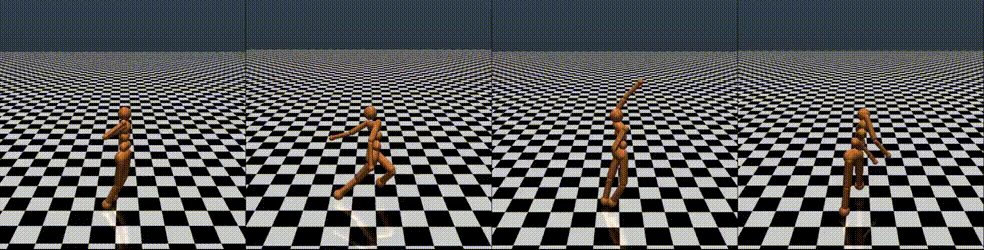
\includegraphics[width=\textwidth]{slika1}
  \caption{Prikaz nekoliko pokušaja čovjekolikog igrača da hoda u \textit{MuJoCo} okruženju}
  \label{slika1}
\end{figure}

\section{Slični radovi}
Vjerojatno najpoznatiju implementaciju ovog algoritma napravio je autor pod nadimkom \textit{SethBling} nazvanu \textit{MarI/O}. Autor je 2015. godine u \textit{YouTube} videu, koji je do sada prikupio više od 7,5 milijuna pregleda, predstavio agenta koji je naučio igrati videoigru \textit{Super Mario World} uz pomoć algoritma NEAT. Na primjeru jednog pokušaja prelaska nivoa (Slika \ref{slika2}) mogu se vidjeti podaci o izvođenju algoritma (na vrhu), vizualizacija agentovog "mozga" (ispod tekstualnih podataka) te stanje igre (pozadina). Agent iz videa nakon 24 sata treniranja uspješno je prešao jedan nivo videoigre.

\begin{figure}
  \centering
  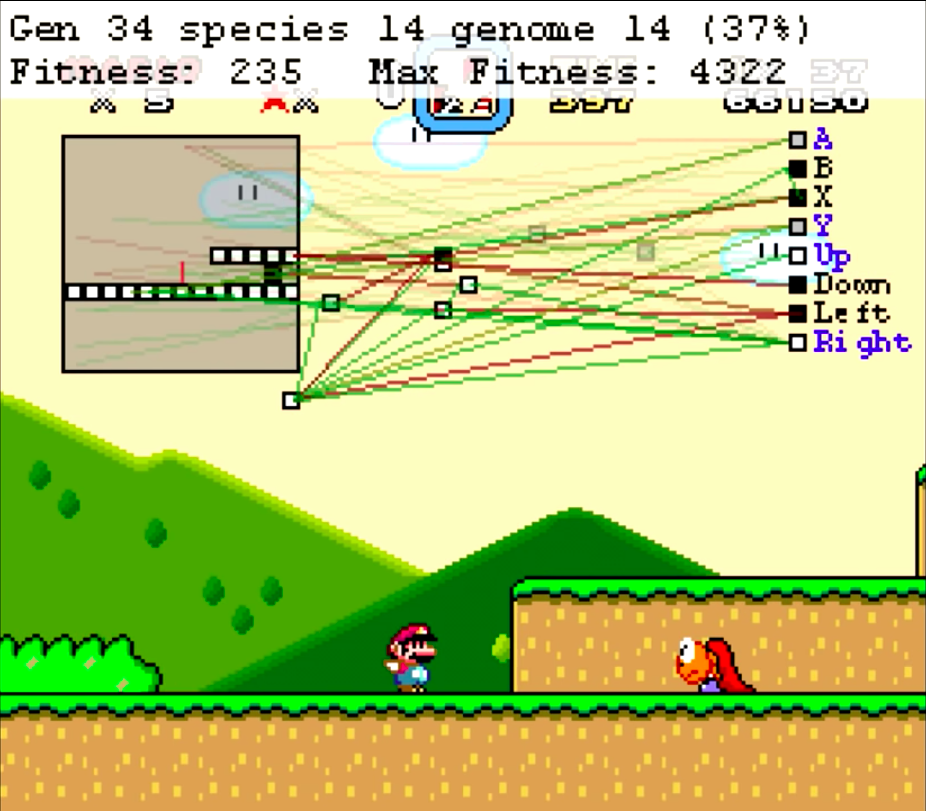
\includegraphics[height=10.5cm]{slika2}
  \caption{Prikaz \textit{MarI/O} agenta kako igra \textit{Super Mario World}}
  \label{slika2}
\end{figure}

Nadalje, u radu \citep{rad6} iz 2013. godine autori Zhen, J.S. i Watson, I. na još jednoj igri prikazuju uporabu algoritma NEAT i njegove varijante u stvarnom vremenu (eng. \textit{real-time NeuroEvolution of Augmenting Topologies}, \textit{rtNEAT}). Igra je bila poseban izazov jer su morali upravljati s više agenata u isto vrijeme, s obzirom da se radi o strategiji u stvarnom vremenu (eng. \textit{Real Time Strategy}, \textit{RTS}). Spomenuta igra je popularna računalna igra \textit{StarCraft: Brood War}. Oba algoritma su koristeći mikromenadžment (eng. \textit{micromanagement}) upravljali jedinicama u igri te su autori pokazali da ove dvije metode postižu bolje rezultate od skriptirane umjetne inteligencije ugrađene u igru. Bitno je primijetiti da je većina dosad spomenutih algoritama ostvarena i ispitana na videoigrama. Računalne igre i umjetna inteligencija dva su pojma koja se sve češće spominju zajedno.

\section{Uloga videoigara u razvoju umjetne inteligencije}
Brzorastuća industrija videoigara stvara sve složenije aproksimacije prirodnih okruženja. Realne simulacije postavljaju odličan okvir unutar kojeg se na djelotvoran i siguran način može razvijati umjetna inteligencija. Nove tehnike i metode mogu se ispitati i ocijeniti u kontroliranim uvjetima prije nego što ih se primijeni na složenije probleme u stvarnom svijetu. Novije računalne igre stvaraju sve veći prostor stanja i akcija, zbog čega predstavljaju veliki izazov u području razvoja umjetne inteligencije. Zbog postepenog rasta složenosti videoigara, odličan su izbor za razvoj umjetne inteligencije zato što je odabirom starijih ili novijih igara moguće lako upravljati težinom problema kojeg se pokušava riješiti. Dosad spomenute videoigre su bile relativno jednostavne, ali neke svjetski najpoznatije istraživačke skupine ispituju svoje algoritme na poznatim novim igrama s velikom kompetitivnom scenom.

Najpoznatiji takav projekt je \textit{OpenAI Five} \citep{rad7}. Njega kontinuirano razvija već spomenuti istraživački tim \textit{OpenAI}. Radi se o sustavu koji je demonstrirao svoj kapacitet na poznatoj računalnoj igri \textit{Dota 2}. To je jedna od najkompetitivnijih igara s velikim brojem igrača i \textit{esport}\footnote{\textit{Esport} je oblik natjecanja koji koristi videoigre. Procijenjeno je da će do 2019. godine 427 milijuna ljudi širem svijeta gledati neki oblik \textit{esporta}.} turnira. \textit{OpenAI Five} je u osmom mjesecu 2017. godine postigao veliki uspjeh i pobijedio nekoliko najboljih \textit{Dota 2 esport} igrača. Važno je napomenuti da je svrha toga bila razviti umjetnu inteligenciju šire primjene, tako da su istim algoritmom na kraju riješili i prethodno neriješen problem u robotici - kontrolu robotske ruke (Slika \ref{slika3}).

\begin{figure}
  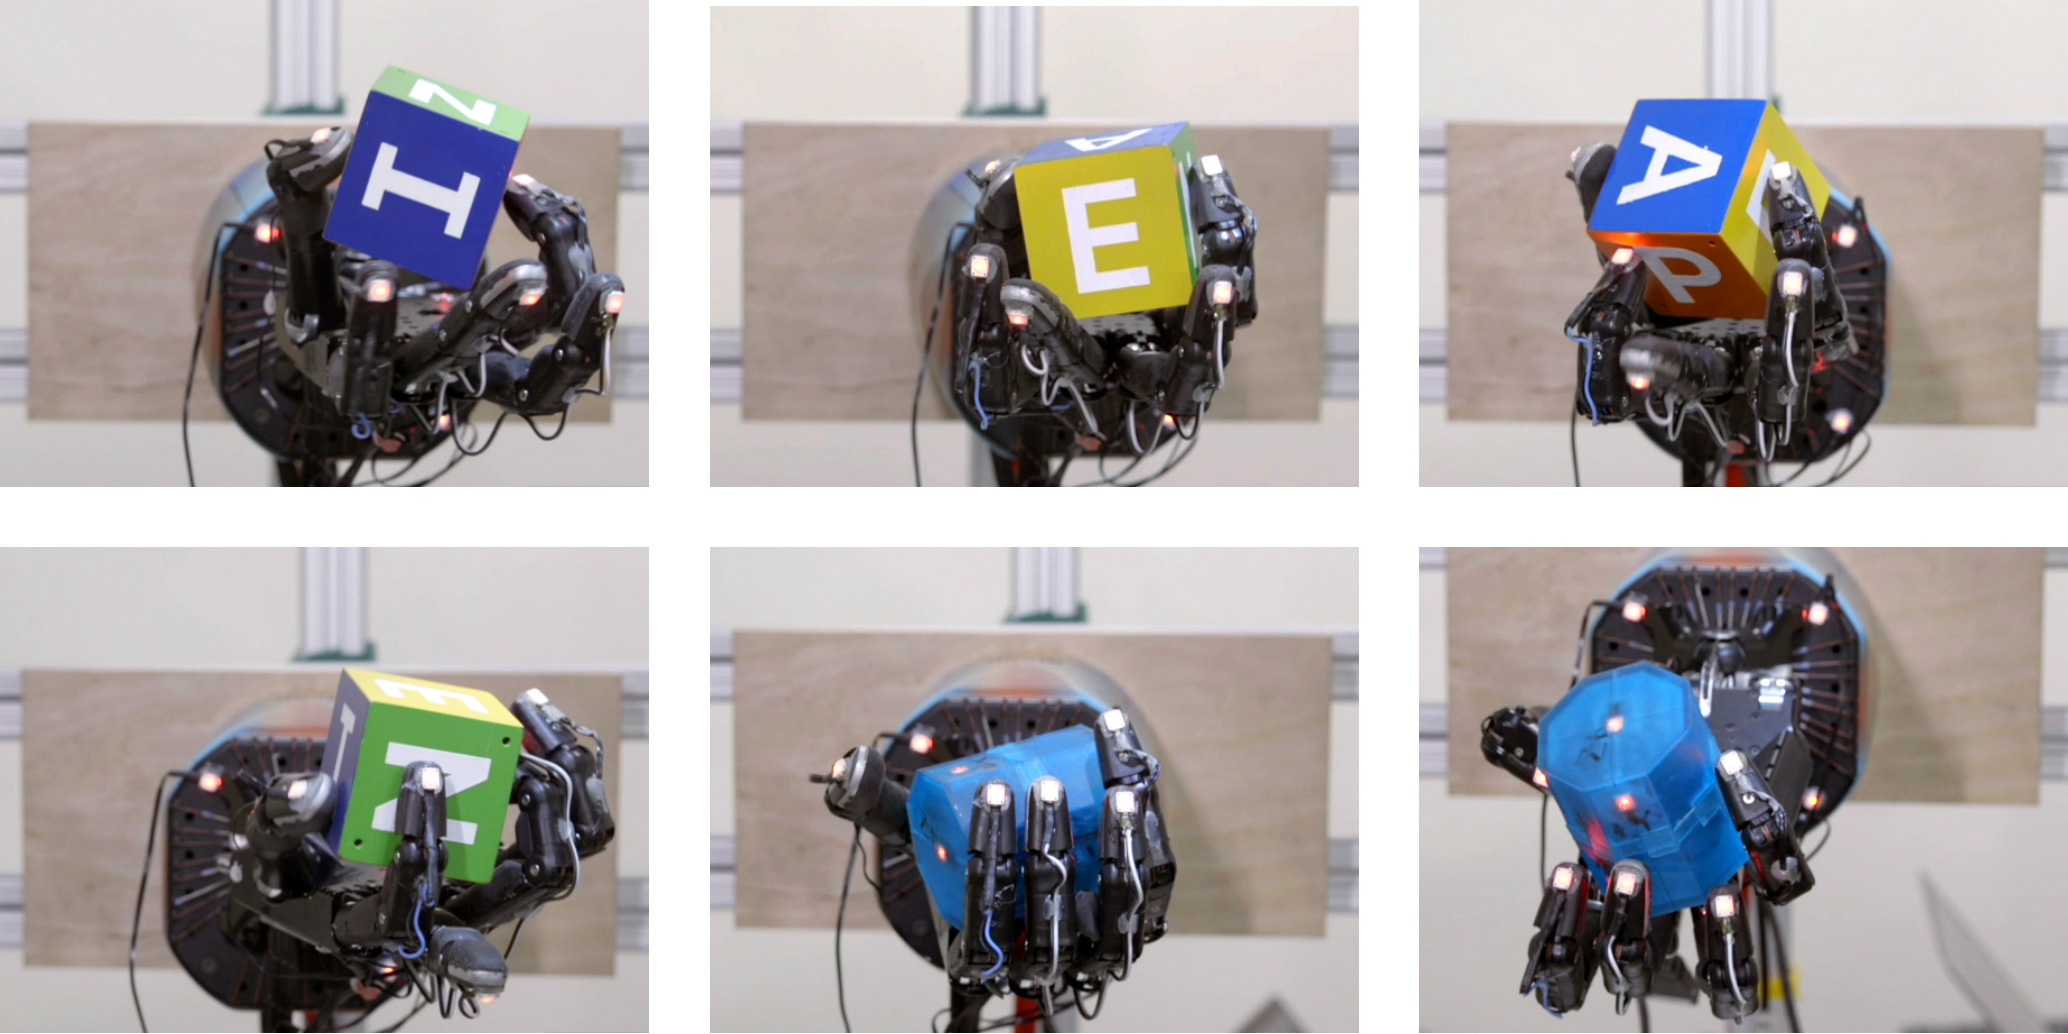
\includegraphics[width=\textwidth]{slika3}
  \caption{Slike robotske ruke kojom upravlja \textit{OpenAI Five}}
  \label{slika3}
\end{figure}

Osim toga, \textit{DeepMind}\footnote{\textit{DeepMind} je \textit{Googleova} tvrtka za razvoj umjetne inteligencije.} nakon svog poznatog projekta \textit{AlphaGo} najavio je da će koristiti RTS igru \textit{StarCraft II} kao okruženje za razvoj umjetne inteligencije. Napravili su ekstenzivan okvir za igru u suradnji s vlasnikom igre, tvrtkom \textit{Blizzard Entertainment}. Ova igra također je jedna od poznatijih na \textit{esport} sceni. \textit{DeepMind} je kratko nakon objave okruženja objavio i rad \citep{rad8} u kojem prezentiraju izazov koji \textit{StarCraft II} predstavlja za područje potpornog učenja. Početkom 2019. godine u video prijenosu prikazali su rezultate koje su postigli te je njihov agent pobijedio dva poznata profesionalna igrača te igre. Ova dva rada pokazala su kako zajednica prepoznaje videoigre kao odličan okvir za razvoj umjetne inteligencije.

U ostatku rada dan je pregled karakteristika i implementacije spomenute vrste neuroevolucijskog algoritma (eng. \textit{NeuroEvolution}, \textit{NE}), kratak opis problema koje se pokušava riješiti u radu te analiza njegove djelotvornosti u treniranju agenata za navedene probleme.

\chapter{Neuroevolucija promjenjivih topologija}
Neuroevolucija promjenjivih topologija (eng. \textit{NeuroEvolution of Augmenting Topologies}, \textit{NEAT}) je genetski algoritam (eng. \textit{Genetic algorithm}, \textit{GA}) za generaciju umjetnih neuronskih mreža (eng. \textit{Artificial Neural Network}, \textit{ANN}). Algoritam mijenja i težine i strukture mreža, pokušavajući tako naći ravnotežu između dobrote razvijenih rješenja i njihove raznolikosti. Bazira se na primjeni tri ključne tehnike: praćenje gena povijesnim oznakama (eng. \textit{history markers}) kako bi se omogućilo križanje topologija, izvršavanje specijacije kako bi se očuvale inovacije te inkrementalan razvoj topologija mreže kako bi se poticala što jednostavnija rješenja.

\section{Zapis gena}
Postupak genetskog enkodiranja napravljen je tako da se odgovarajući geni lako usklade prilikom križanja. Genomi su linearna reprezentacija povezanosti unutar mreže (Slika \ref{slika4}). Svaki genom sadrži listu gena veza (eng. \textit{connection genes}) od kojih svaki referencira dva gena čvora (eng. \textit{node gene}) koji su povezani. Genom sadrži listu ulaznih, skrivenih i izlaznih čvorova koji se mogu spojiti. Svaki gen veze navodi ulazni čvor, izlazni čvor, težinu veze, indikator je li veza uključena te broj inovacije. Inovacijski broj omogućava lako prepoznavanje odgovarajućih gena, a indikator uključenosti veze definira je li veza aktivna ili nije. Ako nije, jedinka će i dalje nositi informacije o toj vezi, ali se ona neće očitovati u fenotipu.

\begin{figure}
  \centering
  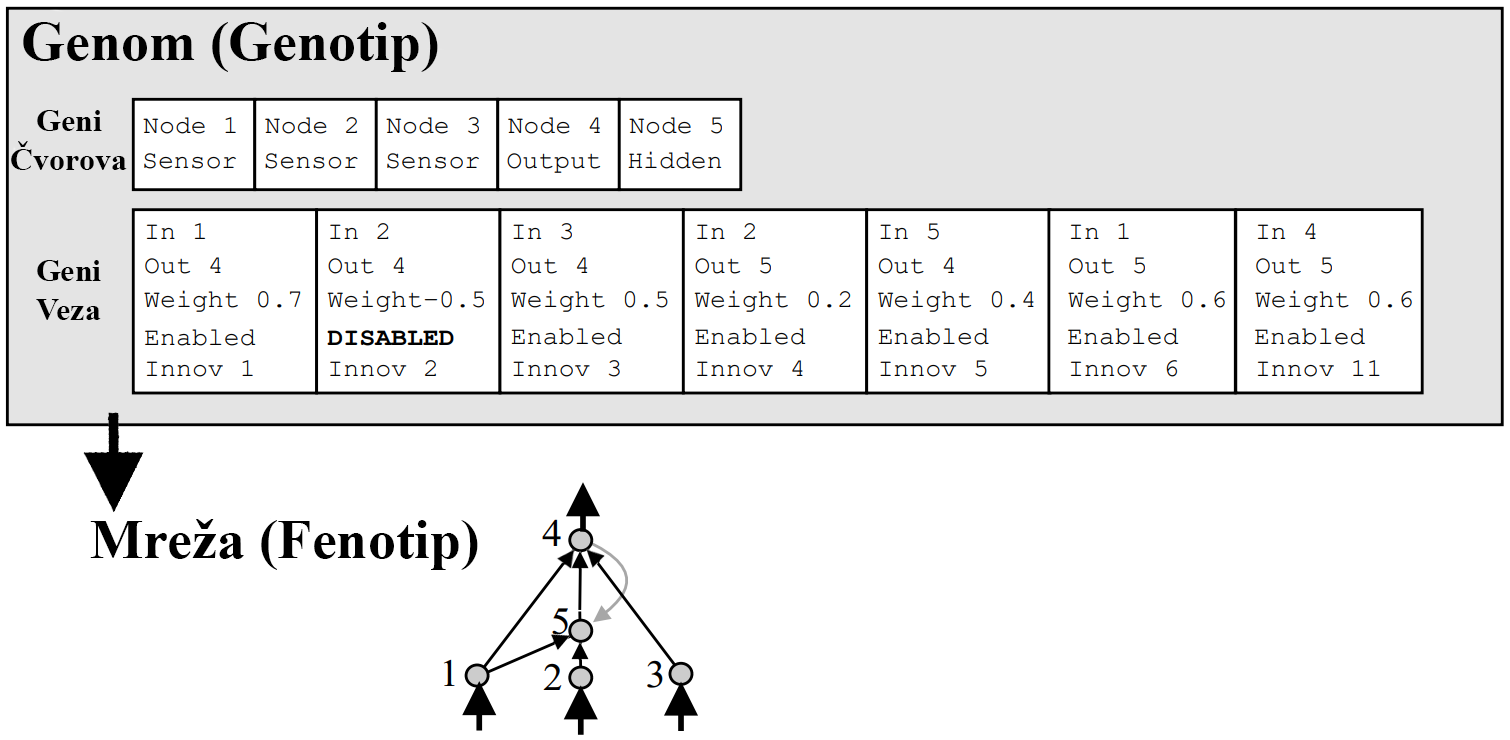
\includegraphics[height=6cm]{slika4}
  \caption{Primjer mapiranja genotipa u fenotip \citep{rad2}}
  \label{slika4}
\end{figure}

Mutacije u algoritmu NEAT mogu promijeniti i težine veza i strukturu mreže. Mutacija težina odvija se kao i kod bilo kojeg neuroevolucijskog sustava, a strukturalna mutacija odvija se na dva načina (Slika \ref{slika5}). Svaka takva mutacija povećava veličinu genoma tako da dodaje gene. U mutaciji dodavanja veze (eng. \textit{add connection mutation}) dodaje se novi gen s nasumično odabranom težinom između dva do tad nepovezana čvora. Nadalje, u mutaciji dodavanja čvora (eng. \textit{add node mutation}) postojeća veza se prepolavlja te se postavlja novi čvor između dva koja su bila povezani tom vezom. Stara veza se isključuje i u genom se dodaju dvije nove veze. Vezi koja ulazi u novonastali čvor težina se postavlja na vrijednost $1$, a vezi koja izlazi iz njega dodjeljuje se težina isključene veze. Kroz mutaciju genomi se postepeno povećavaju. To rezultira mrežama koje na istim mjestima imaju drugačije veze što može izazvati problem prilikom križanja. Osim toga, problem nastaje i zbog genoma različitih veličina. U nastavku je objašnjeno kako algoritam NEAT rješava ovaj problem te kako se ti genomi križaju.

\section{Praćenje gena pomoću povijesnih oznaka}
Sve što sustav treba raditi kako bi znao koji geni su sukladni jest pratiti povijesno ishodište svakog gena. Svaki put kada se pojavi novi gen (kroz strukturnu mutaciju), globalni inovacijski broj (eng. \textit{global innovation number}) se povećava i dodjeljuje tom genu. Samim time, inovacijski broj predstavlja kronologiju svih gena u sustavu. Mogući problem je da iste strukturne inovacije dobiju različite inovacijske brojeve ako su se dogodile u istoj generaciji. U skladu s time, čuvanjem liste inovacija koje su se dogodile u trenutnoj generaciji moguće je osigurati da se svakoj identičnoj mutaciji dodijeli isti inovacijski broj.

\begin{figure}
  \centering
  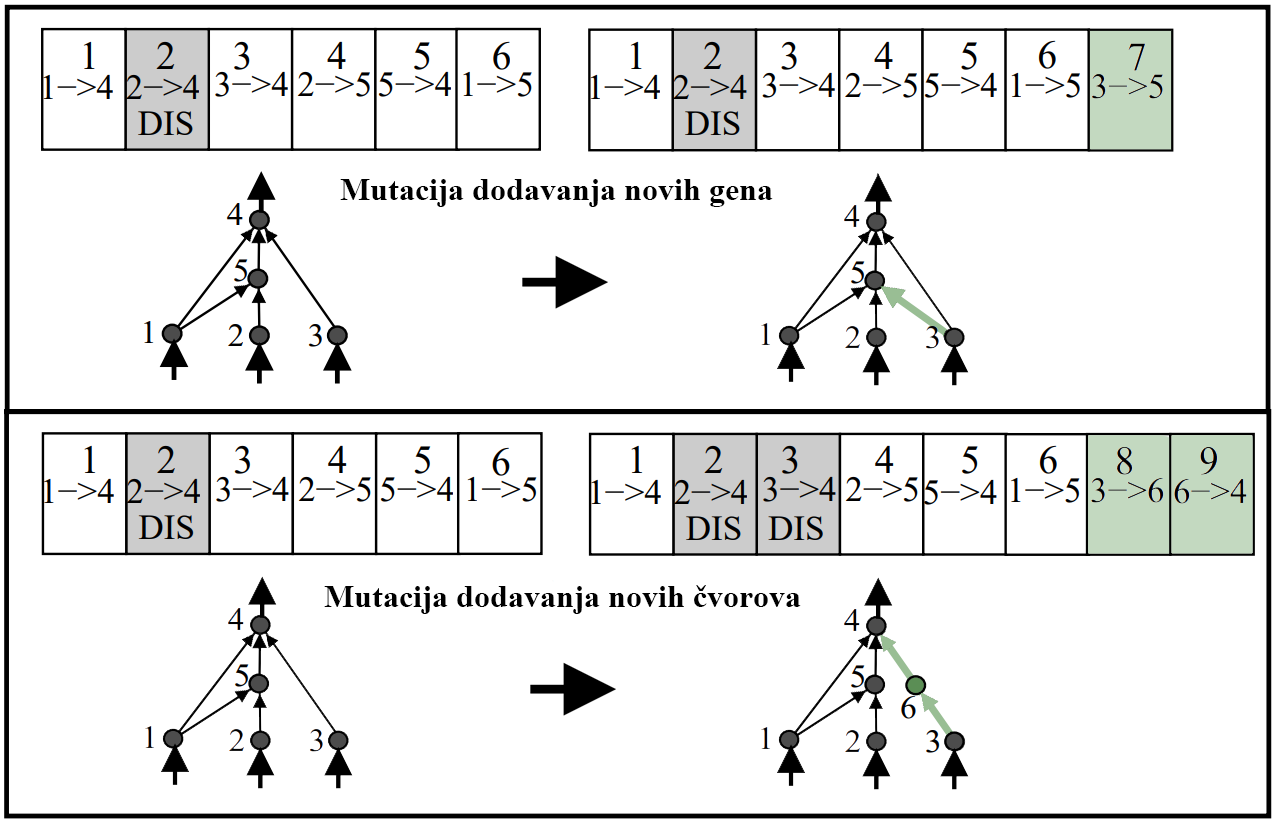
\includegraphics[height=7.5cm]{slika5}
  \caption{Dva tipa strukturalnih mutacija \citep{rad2}}
  \label{slika5}
\end{figure}

Prilikom križanja, geni iz oba genoma s istim inovacijskim brojem se usklade. Geni koji se poklapaju (eng. \textit{matching genes}) nasljeđuju se nasumično, dok se geni koji se ne poklapaju u sredini (eng. \textit{disjoint genes}) i geni koji se ne poklapaju na kraju (eng. \textit{excess genes}) nasljeđuju od roditelja s većom dobrotom. Ako im je dobrota jednaka, dijete nasljeđuje gene od roditelja koji ima jednostavniju strukturu. Dodavanjem novih gena u populaciju i križanjem jedinki sustav formira populaciju raznolikih topologija. Naime, populacija sama po sebi ne može održavati topološke inovacije. Zbog toga što se manje strukture optimiziraju brže od velikih, dodavanje čvorova i veza obično inicijalno smanjuje dobrotu mreže. Stoga, izmijenjene strukture imaju male šanse preživjeti više od jedne generacije, iako inovacije koje uvode mogu biti presudne za rješavanje zadatka. Rješenje je da se inovacije zaštite tako da se populaciju podijeli u vrste, kao što je navedeno u nastavku.

\begin{figure}
  \centering
  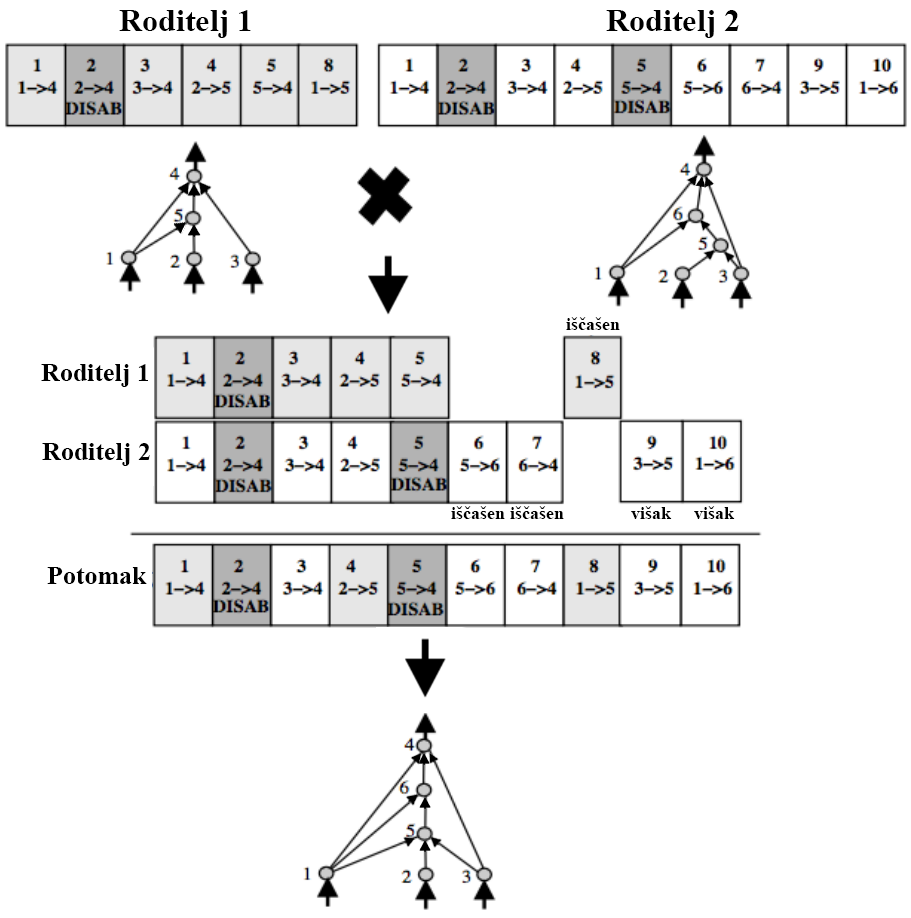
\includegraphics[height=10.5cm]{slika6}
  \caption{Usklađivanje genoma različitih topologija mreža koristeći inovacijske brojeve \citep{rad2}}
  \label{slika6}
\end{figure}

\section{Očuvanje inovacija kroz specijaciju}
Dijeljenjem populacije u vrste u kojima su jedinke sa sličnim topologijama daje jedinkama više vremena da optimiziraju težine. Na ovaj način čuvaju se inovacije koje bi mogle dugoročno pomoći u dostizanju cilja. Način na koji se prepoznaju slične topologije opet je nešto što treba definirati i tu ponovno pomažu povijesne oznake. Broj neusklađenih gena (eng. \textit{disjoint genes}) i viška gena (eng. \textit{excess genes}) između dvije jedinke je mjera njihove sukladnosti. Što je taj broj veći, dijele manje evolucijske povijesti, to jest manje su kompatibilni. Po izrazu iz rada \citep {rad5}, kompatibilna udaljenost (eng. \textit{compatibility distance}) $\delta$ može se izračunati kao funkcija broja viška gena $E$ i neusklađenih gena $D$ te prosječne razlike u težinama usklađenih gena $\bar{W}$, uključujući i isključene veze:

\begin{equation}
\delta = \frac{c_1E}{N} + \frac{c_2D}{N} + c_3\cdot\bar{W}
\label{jednakost1}
\end{equation}

Koeficijenti $c_1$, $c_2$ i $c_3$ su parametri kojima se definira važnost ova tri faktora, a broj $N$ je broj gena u većem genomu i uloga mu je da normalizira izraz. Jednom kada se izračuna udaljenost $\delta$, određuje se pripadnost vrsti pomoću praga kompatibilnosti (eng. \textit{compatibility threshold}) $\delta_t$. Ako je udaljenost $\delta$ između jedinke i predstavnika vrste manja od praga kompatibilnosti $\delta_t$ ta jedinka pripada toj vrsti. Kako bi se tako sortirale jedinke u vrste algoritam cijelo vrijeme treba održavati uređenu listu vrsti. Svaka postojeća vrsta predstavljena je nasumičnim genomom iz prethodne generacije te vrste. Kako se vrste ne bi preklapale, dani genom \textit{g} u trenutnoj generaciji pridijeljen je vrsti prvog reprezentativnog genoma s kojim je kompatibilan. Ako \textit{g} nije kompatibilan ni s jednom postojećom vrstom, stvara se nova vrsta kojoj se \textit{g} postavlja kao reprezentativan uzorak.

Za reprodukcijski mehanizam koristi se eksplicitno dijeljenje dobrote (eng. \textit{explicit fitness sharing}, Goldberg and Richardson, 1987), gdje organizmi u istoj vrsti moraju dijeliti dobrotu. Tako nijedna vrsta ne može postati prevelika, čak i ako su jedinke dobre. Dakle, teško je da će ijedna vrsta preuzeti cijelu populaciju, što je presudno da bi specijacija funkcionirala. Po izrazu iz rada \citep{rad5}, prilagođena dobrota $f_{i}^{'}$ za organizam $i$ računa se sukladno njegovoj udaljenosti $\delta$ od svakog drugog organizma $j$ u populaciji:

\begin{equation}
f_{i}^{'} = \frac{f_i}{\sum_{j=1}^{n} sh(\delta(i,j))}
\label{jednakost2}
\end{equation}

Funkcija dijeljenja $sh$ je $0$ kada je udaljenost $\delta(i,j)$ veća od praga $\delta_t$, inače $sh(\delta(i,j))$ poprima vrijednost $1$. Dakle, suma $\sum_{j=1}^{n}sh(\delta(i,j))$ približno računa broj organizama koji su iste vrste kao i jedinka $i$. Jednom kada se izračuna prilagođena dobrota $f_{i}^{'}$ svih jedinki, uklanjaju se najlošiji organizmi unutar vrsta. Nakon toga, cijela populacija zamjenjuje se potomcima preostalih jedinki u svakoj vrsti. Razlog iz kojeg se provodi specijacija je da bi se očuvale topološke inovacije. Zadnja karakteristika algoritma je da se potraga za rješenjem sustava izvrši što djelotvornije. To se postiže minimiziranjem dimenzionalnosti prostora pretrage.

\section{Minimizacija dimenzionalnosti kroz inkrementalni rast iz minimalne strukture}
Idejna preteča algoritma NEAT, algoritam evolucije topologije i težina umjetne neuronske mreže (eng. \textit{Topology and Weight Evolving Artificial Neural Networks}, \textit{TWEANN}) \citep{rad9}, napunio bi inicijalnu populaciju nasumično generiranim topologijama kako bi potaknuo raznolikost kod završnih rješenja. Algoritam NEAT traži što jednostavnije rješenje i čini pretragu pristranom tako da je inicijalna populacija uniformna te nijedna početna mreža nema skrivenih čvorova. Nova struktura uvodi se postepeno tako što jedinke mutiraju i dobivaju nove čvorove i veze. Novoproširene jedinke preživjet će samo ako imaju visoku dobrotu te se zbog toga može reći da su sve strukturne promjene u algoritmu NEAT opravdane. Budući da je početna struktura populacije jako mala, dimenzionalnost prostora pretrage je smanjena i algoritam NEAT uvijek pretražuje po manje dimenzionalnim domenama od ostalih TWEANN algoritama i neuroevolucijskih sustava s fiksnom topologijom. Zbog toga NEAT ima bolja svojstva nad tim algoritmima, kao što je opisano u radu \citep{rad5}. U sljedećem poglavlju dan je opis implementacije ostvarene u okviru ovog rada.

\chapter{Programsko ostvarenje}
Algoritam koji je ostvaren u okviru ovog rada podijeljen je u nekoliko datoteka i klasa kako bi kod bio pregledniji te lakši za daljnju nadogradnju. Program trenutno podržava izvođenje na nekoliko različitih igara i prikaz bitnih informacija na kraju izvođenja. Svi hiperparametri (eng. \textit{hyperparameters}) odvojeni su u zasebnu datoteku kako bi se olakšalo njihovo podešavanje. Implementacija je napisana u programskom jeziku \textit{Python}. \textit{Python} je trenutno najpopularniji jezik za ostvarenje algoritama strojnog učenja zato što je fleksibilan i pristupačan. Iako je njegova mana to što je sporiji u izvođenju od nekih drugih programskih jezika, postoji veliki broj programskih biblioteka za \textit{Python} čija je implementacija u programskom jeziku \textit{C}, zbog čega je razlika u brzini izvođenja mnogo manja. Prednost je ta što generalno već postoji veliki broj programskih biblioteka koje mogu služiti kao okruženje za implementaciju.

\section{Korištene biblioteke}
Najvažnije programske biblioteke koje se koriste u projektu su tzv. \textit{OpenAI Gym} i \textit{PyGame Learning Environment} (\textit{PLE}). Ove dvije programske biblioteke su okruženja za ispitivanje algoritama potpornog učenja. Podržavaju upravljanje velikim brojem arkadnih i drugih videoigara uz pomoć jednostavnog programskog sučelja (eng. \textit{Application Programming Interface}, \textit{API}). Oba okruženja koriste se tako da se stvori inačica igre na kojoj se pokušava isprobati algoritam. Preko ove inačice pristupa se zapažanjima o trenutnom stanju igre koja su zadana u opisu okruženja. Ova zapažanja služe kao ulaz u neuronsku mrežu koja donosi odluke o sljedećem koraku. Nakon dohvaćanja zapažanja inačici se šalje odluka agenta. Svako okruženje ima definirane akcije koje agent može napraviti u svakom trenutku. Dakle, agent je crna kutija (eng. \textit{black box}) i odabir bilo koje igre iz jednog od okruženja definira broj ulaza i izlaza iz te kutije, tj. neuronske mreže koja je opisana genomom. Nakon što se instanci igre dojavi akcija, okvir se brine da se promjene prikažu na ekranu te vraća nova zapažanja i nagradu koju je agent dobio za tu akciju. Akumuliranjem nagrada za svaki korak na kraju se dobije vrijednost koja definira dobrotu jedinke, to jest agenta.

Na slici \ref{slika20} opisano je sučelje klase koja predstavlja okruženje u okviru paketa \textit{OpenAI gym}. Metoda \textit{make} koristi se za instanciranje željenog okruženja. Metodi se predaje naziv okruženja koji se pokušava instancirati. Kao povratak iz funkcije dobiva se objekt okruženja na kojem se izvode ostale metode. Funkcija \textit{reset} pokreće novu igru u okviru okruženja kojem pripada objekt. Povratak iz funkcije je početno zapažanje nove igre. Kako bi se igra nastavila igrati, potrebno je pozvati metodu \textit{step} sa željenom akcijom. Ova metoda potom vraća i zapažanje novog stanja i nagradu koju je agent dobio za tu akciju. Osim toga, funkcija vraća zastavicu koja označava kraj trenutne igre. Kada agent završi igru ili izgubi pravo za igranjem, zastavica će biti postavljena. Na pozivatelju metode je da pazi da ne poziva \textit{step} nakon što je ta zastavica pozitivna. Zadnja metoda, \textit{render}, ne utječe na tijek izvođenja igre već samo prikazuje trenutno stanje igre na ekranu.

\begin{figure}
  \centering
  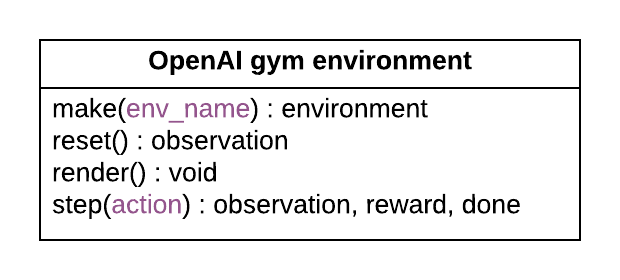
\includegraphics[height=3cm]{slika20}
  \caption{Opis sučelja klase koja predstavlja okruženje u okviru paketa \textit{gym}}
  \label{slika20}
\end{figure}

Programske biblioteke za vizualizaciju grafova i fenotipa su \textit{Matplotlib} i \textit{NetworkX}. \textit{Matplotlib} je najpoznatija programska biblioteka za iscrtavanje grafova u \textit{Pythonu} te olakšava vizualizaciju podataka na kraju izvođenja algoritma. \textit{NetworkX} omogućava prikaz usmjerenih grafova i koristi se za vizualizaciju fenotipa, tj. neuronskih mreža. Programska biblioteka koju je također bitno napomenuti je \textit{NumPy}. \textit{NumPy} je moćan okvir za računanje u \textit{Pythonu} koji je implementiran u programskom jeziku \textit{C} te omogućava brzo i jednostavno baratanje visokodimenzionalnim nizovima. S ovime je zaključen opis vanjskih biblioteka koje su korištene u programskom ostvarenju. U nastavku poglavlja prikazana je struktura projekta koji je ostvaren u okviru ovog rada te su objašnjene neke ključne točke ove implementacije.

\begin{figure}
  \centering
  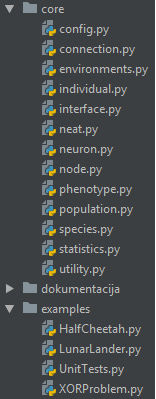
\includegraphics[height=10cm]{slika7}
  \caption{Struktura projekta u programskom okruženju \textit{IntelliJ IDEA}}
  \label{slika7}
\end{figure}

\section{Struktura projekta}
Kao što je navedeno, projekt se sastoji od nekoliko datoteka čija je struktura prikazana na slici \ref{slika7}. Sa slike je moguće razaznati dva glavna paketa. Prvi je \textit{core} u kojem se nalazi implementacija algoritma koja nije direktno vezana za okruženje u kojem se koristi, a drugi je \textit{examples} u kojemu su kratki programi koji pokreću algoritam na različitim problemima koji su podržani. Svaka od datoteka u paketu (Slika \ref{slika7}) sadrži definiciju jedne klase ili apstraktne klase i njenih implementacija. Slika \ref{slika8} vizualni je prikaz strukture klasa u tzv. \textit{Unified Modeling language} (UML) obliku. \textit{Main program} s dijagrama (Slika \ref{slika8}) predstavlja program koji koristi paket \textit{core}. Taj program brine se da stvori instance svih potrebnih klasa i da upravlja izvođenjem algoritma. U ostatku poglavlja prikazani su isječci koda iz paketa \textit{core} bitni za rad programa.

\begin{figure}
  \centering
  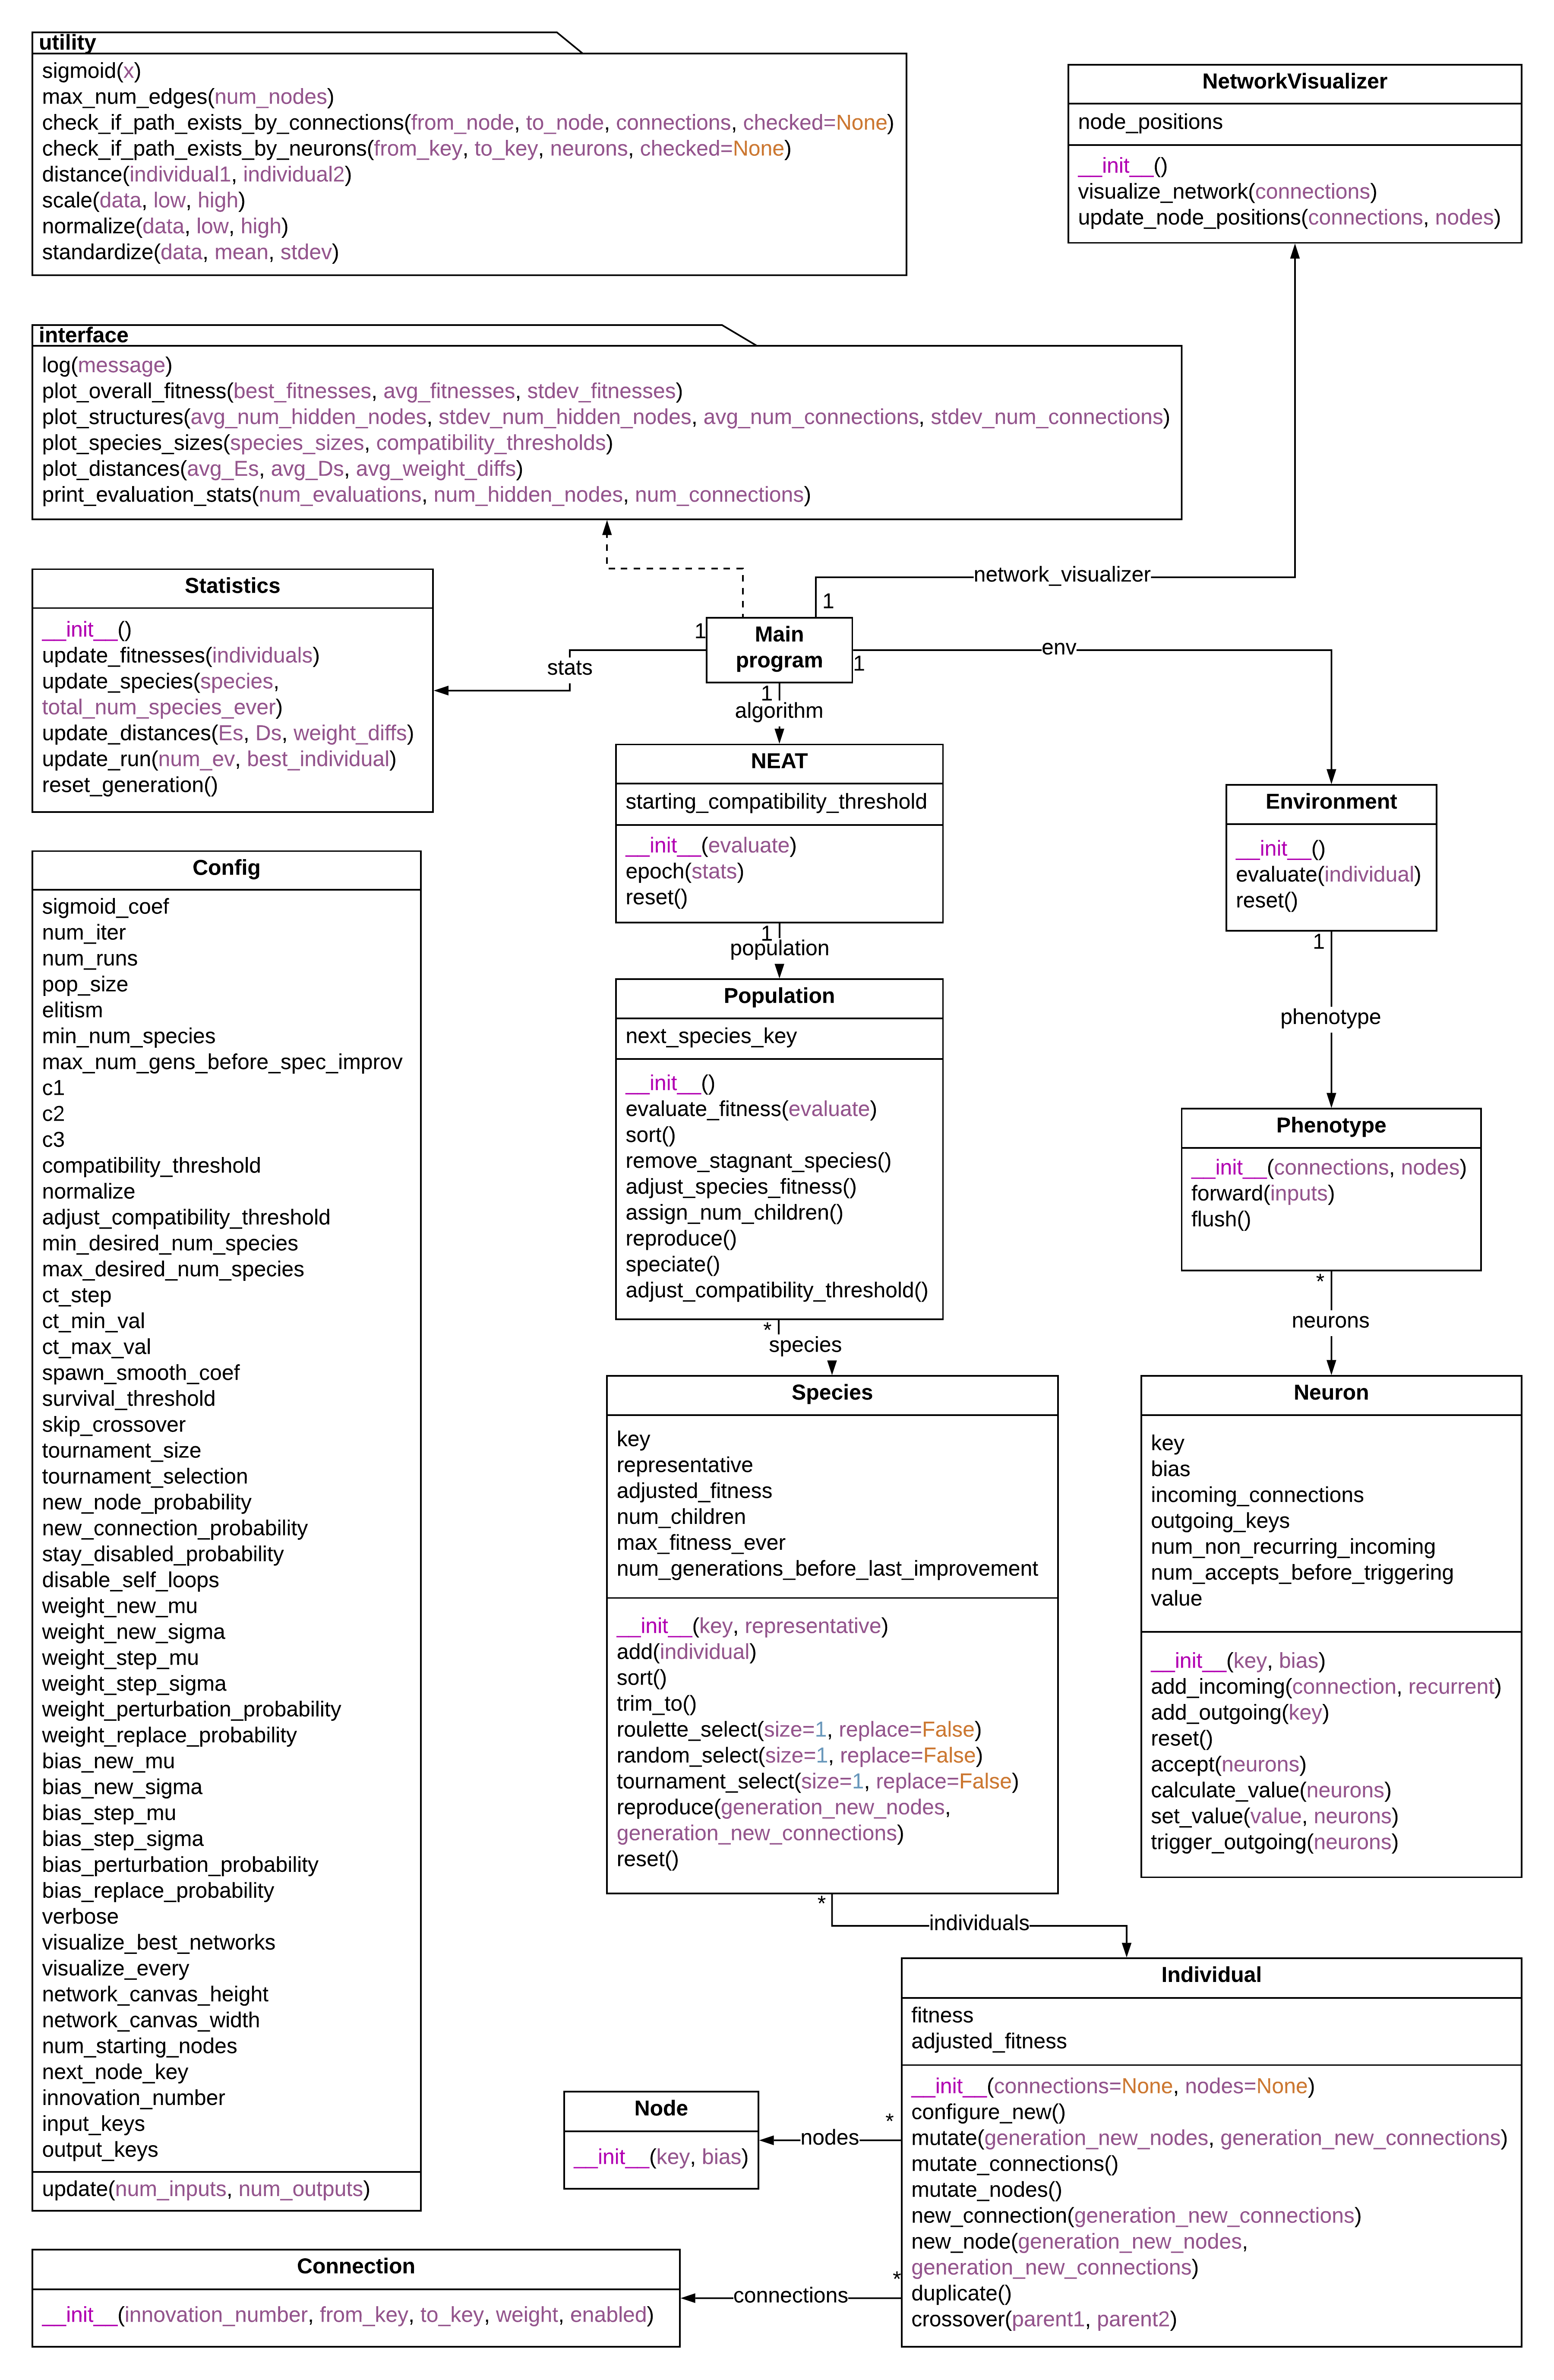
\includegraphics[width=\textwidth]{slika8}
  \caption{UML dijagram paketa \textit{core}}
  \label{slika8}
\end{figure}

\subsection{Klasa \textit{Config}}
Klasa koja je na dijagramu (Slika \ref{slika8}) prikazana kao \textit{Config} sadrži u sebi samo varijable koje su postavljene odmah prilikom instanciranja. Ove varijable upravljaju radom programa i većina ovih vrijednosti su hiperparametri algoritma. Ovako se na jednom mjestu nalaze sve vrijednosti kojima se može upravljati. Iz glavnog programa je onda moguće pisati preko (eng. \textit{overwrite}) postojećih vrijednosti ako se želi mijenjati detalje izvođenja. Instanca se stvara prilikom pokretanja programa i budući da sadrži upute za rad svih aspekata algoritma, tom objektu imaju pristup sve klase unutar paketa.

\subsection{Klasa \textit{NEAT}}
Klasa \textit{NEAT} najapstraktnija je razina izvedbe algoritma. Prilikom instanciranja automatski stvara populaciju veličine definirane u \textit{config} objektu. U kodu \ref{kod1} se vidi tok svake generacije. Prvi korak u svakoj generaciji je evaluiranje dobrote svake jedinke. Ovaj dio algoritma problematičan je zato što se ne može izbjeći evaluaciju svake jedinke u populaciji. Evaluacija u ovakvim problemima je jako skup proces. Opis metode za evaluaciju jedinke nalazi se u \textit{Environment} klasi i na njega utječe način izvedbe okruženja, tj. videoigre koja se igra. Ono što bi pomoglo izvođenju algoritma je da se evaluacija paralelizira. Budući da je evaluacija svake jedinke neovisna, moguće je optimalno iskoristiti raspoložive resurse tako da se jedinke evaluiraju na odvojenim dretvama. Jedino što je potrebno na kraju je prikupiti izlazne vrijednosti metode, dobrote, i pridijeliti ih jedinkama. Ova implementacija ne podržava paralelizaciju zbog nepristupačnosti okvira u kojima su se igre ispitivale. S obzirom na to da je program na računalu s četiri CPU jezgre koristio samo 20\% računalnih resursa, paraleliziranje algoritma uvelike bi ubrzalo izvođenje.

\begin{lstlisting}[frame=single, label=kod1, caption=Izvorni tekst metode \textit{epoch} u klasi \textit{NEAT}]
def epoch(self, stats):
	# evaluate population and track stats
	best_individual = self.population.evaluate_fitness(self.evaluate)
	stats.update_fitnesses(self.population.species)
	stats.update_structures(self.population.species)
	log('\tBest fitness: {:.2f}, Average fitness: {:.2f}'.format(stats.best_fitnesses[-1], stats.avg_fitnesses[-1]))
	log('\tAverage num hidden nodes: {:.2f}, Average num connections: {:.2f}'.format(stats.avg_num_hidden_nodes[-1], stats.avg_num_connections[-1]))

	# sort individuals inside each species and then sort species by their max fitness
	self.population.sort()
	log('\tBest individual is in species {:d}'.format(self.population.species[0].key))

	# remove species that showed no progress in recent generations
	self.population.remove_stagnant_species()

	# normalize adjusted fitness range and assign adjusted fitness to each species
	self.population.adjust_species_fitness()

	# assign children according to adjusted fitness and remove species with no children
	self.population.assign_num_children()

	# copy elites if enabled, remove worst in each species and breed new generation
	children = self.population.reproduce()

	# speciate new individuals and remove empty species
	Es, Ds, weight_diffs = self.population.speciate(children)
	stats.update_species(self.population.species, self.population.next_species_key)
	stats.update_distances(Es, Ds, weight_diffs)
	log('\tNum species is {:d}'.format(len(self.population.species)))
	log('\tAverage distance is {:.2f}'.format(sum(weight_diffs) / len(weight_diffs)))

	# change compatibility threshold if number of species becomes too big or too small
	if config.adjust_compatibility_threshold:
		self.population.adjust_compatibility_threshold()
		log('\tCompatibility threshold is {:.2f}'.format(config.compatibility_threshold))

	return best_individual
\end{lstlisting}

Nadalje, prije ostatka epohe potrebno je sortirati postojeće vrste i jedinke u njima. Sortiranje se izvodi tako da se unutar svake vrste jedinke sortiraju po svojoj dobroti, a onda se vrste sortiraju po njihovoj najvećoj dobroti. Sortiranje olakšava ostatak epohe i iako je inače zahtjevan proces, u usporedbi s evaluacijom zanemariv je zato što kod ovakvih problema postupak evaluacije jedinki uzima puno više vremena, a broj jedinki nije toliko velik da bi sortiranje znatno usporilo rad algoritma. Nakon sortiranja iz populacije se brišu vrste koje dugo nisu vidjele napredak te se onda računaju prilagođene dobrote vrsti i broj jedinki koji će imati u sljedećoj generaciji. Nakon što se pridodijeli broj jedinki koji svaka vrsta može imati, slijedi reprodukcija te specijacija novih jedinki. Ove metode detaljnije su objašnjene u sljedećem potpoglavlju.

\subsection{Klasa \textit{Population}}
Klasa koja predstavlja populaciju, osim klase vrste i jedinke, sadrži logiku algoritma. Klasa \textit{NEAT} je na višoj razini apstrakcije kako bi se kasnije lakše dodavale varijacije algoritma. Osim metoda za evaluaciju populacije i sortiranje, sljedeća metoda koja je bitna za izvođenje algoritma je metoda koja iz populacije briše vrste koje dugo nisu pokazale napredak. Ova metoda opisana je u isječku koda \ref{kod2}. Ukratko, za svaku vrstu se gleda je li njena najbolja dobrota ove generacije bolja od njene dosadašnje najbolje dobrote. Ako je, brojač se resetira. Ako nije, gleda se koliko je generacije prošlo od njenog zadnjeg napretka te ako je prošlo više od broja generacija definiranog u konfiguracijskoj datoteci, ta vrsta se briše. Također, u konfiguracijskoj klasi definirano je i koliki je najmanji broj vrsta koji može ostati nakon brisanja stagnirajućih vrsta. Ako u bilo kojem trenutku preostali broj vrsta postane jednak definiranom, petlja se prekida. Zbog toga što su vrste sortirane silazno prolazak po vrstama zato se izvodi unazad. Tako uvijek se prvo brišu lošije vrste koje stagniraju. Ako se petlja zaustavi ranije zbog toga što je ostao minimalni dopušteni broj vrsta zbog unazadnog prolaska ostat će bolje vrste. Vrijedno je napomenuti da je u originalnoj implementaciji iz rada \citep{rad5} također postojala opcija stagnacije na razini populacije, a ne samo vrsti. U tom slučaju omogućilo bi se razmnožavanje samo dvije najbolje vrste. Ovo je bilo u jednoj od iteracija implementacije, ali je maknuto jer bi takav pristup samo još više usporio algoritam u situacijama kada bi se nasumično postigao visoki rezultat za koji bi populaciji trebalo previše vremena da ga sustigne.

\begin{lstlisting}[frame=single, label=kod2, caption=Izvorni tekst metode \textit{remove\_stagnant\_species} u klasi \textit{Population}]
# assumes species are sorted
def remove_stagnant_species(self):
	# iterate through all species from worst to best
	for spec in reversed(self.species):
		# stop removing stagnant species if number of species is less than or equal to minimum number of species
		if len(self.species) <= config.min_num_species:
			break

		# if species improved reset counter, else increment it
		best_fitness = spec.individuals[0].fitness
		if best_fitness > spec.max_fitness_ever:
			spec.num_gens_before_last_improv = 0
			spec.max_fitness_ever = best_fitness
		else:
			spec.num_gens_before_last_improv += 1

			# if species hasn't improved in a long time remove it from the population
			if spec.num_gens_before_last_improv > config.max_num_gens_before_spec_improv:
				log('\t\tRemoving stagnant species {:d} after {:d} generations without improvement'.format(spec.key, spec.num_gens_before_last_improv))
				self.species.remove(spec)
\end{lstlisting}

Nakon eliminacije stagnirajućih vrsta slijedi prvi korak pripreme populacije za reprodukciju. Kako bi se odredilo koliko će se potomaka pridijeliti svakoj vrsti prvo se mora izračunati prilagođena dobrota svake vrste. U originalnom radu \citep{rad5} ovo je izvedeno tako da se računala prilagođena dobrota za svaku jedinu po jednakosti \ref{jednakost2} te se onda prilagođena dobrota za vrstu gledala kao zbroj prilagođenih dobrota njenih jedinki. S obzirom da bi za računanje prilagođene dobrote jedinke trebalo gledati njenu udaljenost od svake jedinke u populaciji, postupak je pojednostavljen. Tako se u tom slučaju dobrota ne dijeli s brojem jedinki koji su unutar praga udaljenosti od iste, nego se dijeli s brojem jedinki unutar vrste kojoj jedinka pripada. Sukladno tome, zbroj prilagođenih dobrota svih jedinki unutar vrste zapravo bi dalo prosječnu dobrotu jedinki vrste. Zbog toga u metodi odmah računa prilagođena dobrota vrste, jer se ionako koristi samo u tom kontekstu. Također, zbog načina na koji se koristi ona u originalnom radu nikada nije smjela biti negativna. Kako bi se to ograničenje izbjeglo u implementaciju je dodana normalizacija. Stoga, u metodi se prvo računa najmanja i najveća dobrota u generaciji, kako bi se kasnije koristeći taj raspon mogla normalizirati prosječna dobrota vrste. Novodobivena vrijednost sprema se u objekt vrste kao prilagođena dobrota.

\begin{lstlisting}[frame=single, label=kod3, caption=Izvorni tekst metode \textit{adjust\_species\_fitness} u klasi \textit{Population}]
def adjust_species_fitness(self):
	# find minimum and maximum fitness for normalization
	min_fitness = math.inf
	max_fitness = -math.inf
	for spec in self.species:
		for individual in spec.individuals:
			if individual.fitness < min_fitness:
				min_fitness = individual.fitness

			if individual.fitness > max_fitness:
				max_fitness = individual.fitness

	# define fitness range
	fitness_range = max(abs(max_fitness - min_fitness), 1.0)

	for spec in self.species:
		# calculate species mean fitness
		mean_fitness = sum([individual.fitness for individual in spec.individuals]) / len(spec.individuals)
		# set adjusted fitness as normalized mean fitness
		spec.adjusted_fitness = (mean_fitness - min_fitness) / fitness_range
\end{lstlisting}

Izračunate prilagođene dobrote vrsti bitne su za sljedeći korak algoritma koji se izvodi pomoću metode opisane u isječku koda \ref{kod4}. Metoda \textit{assign\_num\_children} pridjeljuje svakoj vrsti broj potomaka za reprodukciju u sljedećem koraku. Svaka vrsta dobiva pravo na broj potomaka proporcionalan svojoj prilagođenoj dobroti. Bitno je da zbroj svih potomaka na kraju bude otprilike jednak veličini vrste definiranoj u postavkama. Hiperparametar za elitizam ne dopušta da se vrsti pridijeli manje od definiranog broja potomaka. Na ovaj način svaka vrsta sigurno će imati barem jednog potomka kako bi imala priliku razviti se, a na detekciji stagnacije je da ukloni vrste kojima treba previše vremena zbog zapinjanja u lokalnom optimumu.

\begin{lstlisting}[frame=single, label=kod4, caption=Izvorni tekst metode \textit{assign\_num\_children} u klasi \textit{Population}]
def assign_num_children(self):
	total_spawn = 0
	adjusted_fitness_sum = sum([spec.adjusted_fitness for spec in self.species])

	for spec in self.species:
		adjusted_fitness = spec.adjusted_fitness
		size = len(spec.individuals)

		# calculate potential number of children proportionally to species adjusted fitness
		potential_size = max(config.elitism, adjusted_fitness / adjusted_fitness_sum * config.pop_size)
		# calculate difference between current size and potential number of children
		size_delta = potential_size - size
		# set number of children somewhere between current and potential size depending on smoothing coefficient
		num_children = size + round(size_delta * config.spawn_smooth_coef)

		spec.num_children = num_children
		total_spawn += num_children

	# calculate coefficient with which we will normalize all number of children
	norm = config.pop_size / total_spawn

	for spec in self.species:
		# by normalizing we assure population size will always be as close to defined as possible
		spec.num_children = max(config.elitism, round(spec.num_children * norm))

	# if there is no elitism in species it is possible some have 0 children assigned, remove those species if so
	if config.elitism == 0:
		log('\t\tRemoving species {:d} because no children were assigned'.format(self.spec.key))
		self.species = [spec for spec in self.species if spec.num_children > 0]
\end{lstlisting}

Reprodukcija se odvija tako da objekt populacije sakupi sve jedinke koje su stvorile pojedine vrste. Klasa populacije samo poziva metodu za reprodukciju iz klase vrste, zbog toga što se reprodukcija odvija unutar vrste. Ta metoda objašnjena je u sljedećem podpoglavlju. Nakon reprodukcije, nove jedinke treba odvojiti u vrste. Ovo je prikazano u isječku \ref{kod5}. Implementacija je jednostavna, iterira se po novim jedinkama i računa se njihova udaljenost do svakog predstavnika vrste. Jedinka se stavlja u vrstu prvog predstavnika s kojim je kompatibilna. Ako je udaljenost jedinke od svih predstavnika veća od praga definiranog u postavkama, stvara se nova vrsta te se tu jedinku postavlja kao predstavnika te nove vrste.

\begin{lstlisting}[frame=single, label=kod5, caption=Izvorni tekst metode \textit{speciate} u klasi \textit{Population}]
def speciate(self, children):
	# assign every individual to a species
	for individual in children:
		placed = False

		Es = []
		Ds = []
		weight_diffs = []

		# first see if individual is compatible with any existing species
		for spec in self.species:
			dist_from_repr, E, D, weight_diff = utility.distance(individual, spec.representative)

			Es.append(E)
			Ds.append(D)
			weight_diffs.append(weight_diff)

			# if distance from species representative is smaller than threshold add individual to that species
			if dist_from_repr <= config.compatibility_threshold:
				spec.add(individual)
				placed = True
				break

		# if individual is not placed to any existing species create new species and set it as representative
		if not placed:
			new_spec = Species(self.next_species_key, individual)
			self.species.append(new_spec)
			self.next_species_key += 1

	# log empty species
	for spec in self.species:
		if len(spec.individuals) == 0:
			log('\t\tSpecies {:d} is empty after speciation'.format(spec.key))

	# delete any species that is empty after speciation
	self.species = [spec for spec in self.species if len(spec.individuals) > 0]

	return Es, Ds, weight_diffs
\end{lstlisting}

Specijacija je dobra zato što omogućuje jedinkama da se bore za prevlast s jedinkama koje su im slične. U ovakvom algoritmu potrebno je imati neki način kojim se potiče razvoj novih struktura, budući da je to jedna od osnovnih premisa ovog algoritma. S obzirom na to da je prag udaljenosti hiperparametar koji treba unaprijed podesiti, jedan od problema koji se može dogoditi je da vrste budu ili prevelike ili premale. Ako su vrste premale jedinke će biti preslične i algoritma neće moći dobro pretraživati prostor rješenja. S druge strane, ako je broj vrsta premali ugušit će se strukturalne promjene koje inicijalno imaju loše težine, ali bi dugoročno mogle biti korisne. Stoga je dodana metoda koja prilagođava prag udaljenosti ovisno o trenutnom broju vrsti i željenom broju vrsti. Ovo smanjuje pritisak odabira dobrog praga, ali stvara novi hiperparametar. Ispitivanjem ponašanja algoritma pokazalo se da je taj hiperparametar robusniji i lakše ga je dobro procijeniti. Metoda je prikazana u isječku \ref{kod6} i gleda je li broj vrsta manji od minimalnog ili veći od maksimalnog traženog. Ako je, prag će se ili smanjiti ili povećati. Ako je broj vrsta unutar željenog raspona ne događa se ništa. Također, moguće je da se u prvom dijelu algoritma prag previše smanji ili poveća, dok algoritam još zbog mutacije ni ne dobije priliku stvoriti dovoljno različitih jedinki. Kako bi se izbjegla eksplozija broja vrsti, u slučaju da je pređe, novu vrijednost praga na kraju je potrebno zalijepiti na minimalnu ili maksimalnu moguću vrijednost. U sljedećem poglavlju na primjeru jednog od problema prikazan je utjecaj ove metode na brzinu algoritma.

\begin{lstlisting}[frame=single, label=kod6, caption=Izvorni tekst metode \textit{adjust\_compatibility\_threshold} u klasi \textit{Population}]
def adjust_compatibility_threshold(self):
	num_species = len(self.species)

	# calculate compatibility threshold modifier depending on current number of species
	delta = 0
	if num_species > config.max_desired_num_species:
		delta = config.ct_step
	elif num_species < config.min_desired_num_species:
		delta = -config.ct_step

	# adjust current value with calculated modifier but make sure it doesn't go over defined boundaries
	new_value = config.compatibility_threshold + delta
	config.compatibility_threshold = np.clip(new_value, config.ct_min_val, config.ct_max_val)
\end{lstlisting}

\subsection{Klasa \textit{Species}}
Ova klasa služi za praćenje jedinki unutar jedne vrste i za njihovo lako upravljanje. Osim osnovnih metoda kao što su dodavanje jedinki u vrstu, sortiranje, skraćivanje i nasumične selekcije, dodana je još jedna vrsta selekcije koja nije spomenuta u originalnom radu \citep{rad5}. Selekcija koja se koristila u tom radu je selekcija analogna ruletu (eng. \textit{roulette wheel selection}). Ona odabire nasumično gdje je vjerojatnost odabira jedinke proporcionalna s njenom dobrotom, ali je predstavljala probleme zbog toga što se s njom ne mogu koristiti negativne vrijednosti dobrote. U izvođenjima je nasumična selekcija pokazala bolje rezultate. Ali, selekcija o kojoj se tu priča nije ni nasumična. Selekcija s kojom su se u ispitivanjima uspoređeni rezultati je turnirska selekcija (Kod \ref{kod7}). Ova selekcija odabire $k$ jedinki, gdje je $k$ unaprijed definiran u postavkama kao hiperparametar i označava veličinu turnira. Nakon odabira $k$ jedinki samo one se uspoređuju i pobjeđuje prva, tj. prvih $n$, gdje je $n$ broj jedinki koje se žele zadržati u populaciji ili reproducirati. Zbog toga, veći $k$ znači veći pritisak na jedinke, jer će slabije jedinke imati manju šansu za pobjedu što je veći turnir. Rezultati ispitivanja nalaze se u sljedećem poglavlju.

\begin{lstlisting}[frame=single, label=kod7, caption=Izvorni tekst metode \textit{tournament\_select} u klasi \textit{Species}]
# returns single element, tuple or a list based on selection size
def tournament_select(self, size=1, replace=False):
	assert size < config.tournament_size, 'Size must be smaller than tournament size for selection to have effect'

	# randomly select individuals that will be inside the tournament and sort them from best to worst
	tournament = self.random_select(config.tournament_size, replace)
	tournament.sort(key=lambda x: -x.fitness)

	# we return individuals from the top because they are the winners
	if size == 1:
		return tournament[0]
	if size == 2:
		return tournament[0], tournament[1]
	else:
		return tournament[:size]
\end{lstlisting}

Osim selekcije, važna metoda unutar ove klase je metoda za reprodukciju (Kod \ref{kod8}). Ova metoda pretpostavlja da je vrsti već pridodijeljen broj potomaka. Metoda kao argument prima dvije varijable koje se mogu vidjeti u isječku koda. Te varijable su rječnici (eng. \textit{dictionary}) koji pohranjuju generacijske inovacije. Ovo je potrebno zato što je vezama između istih čvorova unutar iste generacije potrebno dati isti inovacijski broj. Također, potrebno je prepoznati i nove čvorove između ista dva postojeća. S obzirom na to da se trenutno te promjene prate samo na razini jedne generacije, vrijedi razmotriti opciju u kojoj se ove strukturalne promjene prate na razini svih generacija. Tako bi nove veze između istih čvorova uvijek imale isti inovacijski broj, a ne samo ako su nastale u istoj generaciji.

Prije početka križanja jedinki, vrsta prvo prosljeđuje najbolje jedinke u sljedeću generaciju. Ova karakteristika zove se elitizam (eng. \textit{elitism}). Najčešće se u sljedeću generaciju direktno prenosi samo jedna jedinka, ali njihov broj se može podesiti u postavkama. Nakon elitnih jedinki, brišu se najlošije jedinke koje neće imati pravo imati potomke. Postotak preživljavanja definiran je kao hiperparametar. Iako mali postotak preživljavanja može biti loš jer se tako isto guše moguće korisne strukturalne promjene, do sada je nasumična selekcija i mali postotak preživljavanja pokazao bolje rezultate od turnirske selekcije. Vrijedi isprobati turnirsku selekciju s velikim pritiskom kako bi se dobio sličan efekt ovome, ali na logičniji način. Ova metoda uzima u obzir da su jedinke sortirane, tako da nakon prorjeđivanja ostanu samo najbolje. Nakon toga započinje reprodukcija. Za svaku novu jedinku iznova se gleda kolika je vjerojatnost da se jedinka dobije kloniranjem jedne jedinke ili križanjem dvije. Ako se preskače križanje odabire se jedna jedinka i ona se klonira i mutira, inače se odabiru dvije i nakon križanja mutira se dobivena jedinka. Način selekcije takvih jedinki definiran je u postavkama i može biti obavljen nasumičnom ili turnirskom selekcijom. Kada se prikupi broj jedinki veličine dodijeljenog broja potomaka metoda završava i jedinke se prosljeđuju pozivatelju metode.

\begin{lstlisting}[frame=single, label=kod8, caption=Izvorni tekst metode \textit{reproduce} u klasi \textit{Species}]
# assumes individuals are sorted
def reproduce(self, generation_new_nodes, generation_new_connections):
	size = len(self.individuals)

	children = []

	# if elitism is enabled automatically forward best individuals to next generation
	num_elites = min(config.elitism, size)
	for i in range(num_elites):
		child = self.individuals[i].duplicate()
		children.append(child)
		self.num_children -= 1

	# remove bottom part of the individuals which are not allowed to reproduce
	num_surviving = max(2, math.ceil(config.survival_threshold * size))
	self.trim_to(num_surviving)

	size = len(self.individuals)
	# create children until assigned cap is reached
	while self.num_children > 0:
		# select two parents for crossover or duplicate a single individual
		if random.random() < config.skip_crossover or size < 2:
			parent = self.random_select()
			child = parent.duplicate()
		else:
			if not config.tournament_selection or size < config.tournament_size:
				parent1, parent2 = self.random_select(2)
			else:
				parent1, parent2 = self.tournament_select(2)

			child = crossover(parent1, parent2)

		# after we have a child, mutate it
		child.mutate(generation_new_nodes, generation_new_connections)

		children.append(child)
		self.num_children -= 1

	# reset species, remove all individuals and set a random one as a representative
	self.reset()

	return children
\end{lstlisting}

\subsection{Klasa \textit{Individual}}
Klasa koja predstavlja jedinku ujedno sadrži u sebi i genom. Zbog toga, ako prilikom instanciranja nisu proslijeđene veze i čvorovi, jedinka mora stvoriti nove. Ovo je prikazano u isječku \ref{kod9}. Za svaki ulaz i izlaz stvara se novi čvor s nasumičnom pristranošću (eng. \textit{bias}). Nakon toga između svih ulaznih i izlaznih čvorova stvaraju se veze s nasumičnom težinom. U originalnom radu \citep{rad5} čvorovi nemaju težinu, nego su autori u ispitivanjima imali još jedan ulaz u mrežu koji je uvijek imao vrijednost $1$. U ispitivanjima se pokazalo da je bolje imati pristranost ugrađenu u čvor koji onda mutira slično kao težina veze. Zbog toga, zapis čvora se također smatra dijelom genoma i čvorovi se prate jedinstvenim ključem isto kao i veze inovacijskim brojem. Naravno, prilikom križanja dijete roditelja preuzima karakteristike čvorova isto kao i težina.

\begin{lstlisting}[frame=single, label=kod9, caption=Izvorni tekst metode \textit{configure\_new} u klasi \textit{Individual}]
def configure_new(self):
	# create a node for every input and output defined by the problem
	for key in config.input_keys + config.output_keys:
		# pick random bias value with gaussian distribution
		bias = random.gauss(config.bias_new_mu, config.bias_new_sigma)
		node = Node(key, bias)
		self.nodes[key] = node

	next_innovation_number = 0
	# fully connect inputs and outputs, i.e. create a connection between every input and output node
	for input_key in config.input_keys:
		for output_key in config.output_keys:
			# pick random connection weight value with gaussian distribution
			new_connection = Connection(next_innovation_number, input_key, output_key, random.gauss(config.weight_new_mu, config.weight_new_sigma), True)
			self.connections[next_innovation_number] = new_connection
			next_innovation_number += 1
\end{lstlisting}

Mutacija je bitna kod genetskih algoritama zato što osim križanja određuje kako se populacija kreće po prostoru rješenja. Kao što je vidljivo u isječku \ref{kod10}, prilikom mutiranja jedinke moguće su tri vrste mutacije. Zbog dodane pristranosti u čvorovima, u ovoj implementaciji postoji i četvrta vrsta mutacije, mutacija čvorova. U postavkama je definirano kolike su vjerojatnosti svake od mutacija.

\begin{lstlisting}[frame=single, label=kod10, caption=Izvorni tekst metode \textit{mutate} u klasi \textit{Individual}]
def mutate(self, generation_new_nodes, generation_new_connections):
	# new connection mutation
	if random.random() < config.new_connection_probability:
		self.new_connection(generation_new_connections)

	# new node mutation
	if random.random() < config.new_node_probability:
		self.new_node(generation_new_nodes, generation_new_connections)

	# connection weight and node bias mutations
	self.mutate_connections()
	self.mutate_nodes()
\end{lstlisting}

Mutacije veza i čvorova (Kod \ref{kod11}) su jednostavne, iterira se po čvorovima ili vezama i ovisno o vjerojatnostima zadanima u postavkama vrijednosti se perturbiraju ili ih se resetira na nove nasumične vrijednosti.

\begin{lstlisting}[frame=single, label=kod11, caption=Izvorni tekst metodi \textit{mutate\_connections} i \textit{mutate\_nodes} u klasi \textit{Individual}]
def mutate_connections(self):
	# go through all connections and either adjust weight by a small amount or assign a new random one
	for connection in self.connections.values():
		r = random.random()
		if r < config.weight_perturbation_probability:
			connection.weight += random.gauss(config.weight_step_mu, config.weight_step_sigma)
		elif r < config.weight_perturbation_probability + config.weight_replace_probability:
			connection.weight = random.gauss(config.weight_new_mu, config.weight_new_sigma)

def mutate_nodes(self):
	# go through all nodes and either adjust bias by a small amount or assign a new random one
	for node in self.nodes.values():
		r = random.random()
		if r < config.bias_perturbation_probability:
			node.bias += random.gauss(config.bias_step_mu, config.bias_step_sigma)
		elif r < config.bias_perturbation_probability + config.bias_replace_probability:
			node.bias = random.gauss(config.bias_new_mu, config.bias_new_sigma)
\end{lstlisting}

Stvaranje nove veze je potencijalno najzahtjevnija metoda (kod \ref{kod12}. Potrebno je paziti da se ne pokuša stvoriti veza kojom bi graf postao kružni. Zbog jednostavnosti poželjno je da neuronska mreža bude samo unaprijedna (eng. \textit{feedforward}). Moguće je jedino u postavkama omogućiti stvaranje povratnih veza. Te veze bi započinjale i završavale u istom čvoru. Uz povratnu vezu čvor bi mogao uzeti u obzir svoje prethodne vrijednosti te bi se tako uvela memorija u neuronsku mrežu. Ovo je potrebno u problemima koji nemaju Markovljevo svojstvo (non-Markovian property). Kako bi se spriječila beskonačna petlja na početku metode prvo se provjerava je li uopće moguće dodati novu vezu. Ako je, pokušavaju se odabrati dva čvora takva da veza između njih već ne postoji. Ako se primijeti da bi novonastala veza stvorila kružnu vezu, usmjerenje veze se obrne. Jednom kada je to obavljeno, pomoću rječnika koji smo primili kao argument gleda se je li takva strukturalna promjena već nastala. Sukladno tome daje joj se ili prikladni inovacijski broj ili joj se pridodaje novi i strukturalna promjena se sprema za buduće mutacije. Nova veza ima nasumičnu težinu.

\begin{lstlisting}[frame=single, label=kod12, caption=Izvorni tekst metode \textit{new\_connection} u klasi \textit{Individual}]
def new_connection(self, generation_new_connections):
	node_keys = list(self.nodes.keys())
	num_nodes = len(node_keys)
	num_connections = len(self.connections.values())
	num_inputs = len(config.input_keys)
	num_outputs = len(config.output_keys)

	# exit if it is not possible to create any new connections
	if num_connections == utility.max_num_edges(num_nodes) - (utility.max_num_edges(num_inputs) + utility.max_num_edges(num_outputs)):
		return

	while True:
		# pick two random nodes
		node1_key = random.choice(node_keys[num_inputs + num_outputs:])
		node2_key = random.choice(node_keys)

		# try again if chosen nodes are the same and self loops are disabled
		if config.disable_self_loops and node1_key == node2_key:
			continue

		# try again if there is already an existing connection between chosen nodes
		existing_connections = [c for c in self.connections.values() if c.from_key == node1_key and c.to_key == node2_key or c.from_key == node2_key and c.to_key == node1_key]
		if existing_connections:
			continue

		# switch node positions if adding this link would make network recurrent
		if node2_key in config.input_keys or utility.check_if_path_exists_by_connections(node2_key, node1_key, self.connections) or (node2_key, node1_key) in generation_new_connections:
			temp = node1_key
			node1_key = node2_key
			node2_key = temp

		# assign new innovation number or assign existing if structural innovation has already occurred
		key_pair = (node1_key, node2_key)
		if key_pair in generation_new_connections:
			innovation_number = generation_new_connections[key_pair]
		else:
			innovation_number = config.innovation_number
			generation_new_connections[key_pair] = innovation_number
			config.innovation_number += 1

		# create new connection with random weight
		new_connection = Connection(innovation_number, node1_key, node2_key, random.gauss(config.weight_new_mu, config.weight_new_sigma), True)
		self.connections[innovation_number] = new_connection
		return
\end{lstlisting}

Dodavanje novog čvora ima nešto jednostavniju implementaciju (Kod \ref{kod13}). Potrebno je samo iz liste veza izabrati jednu nasumično. U predanim generacijskim inovacijama gleda se je li čvor na ovom mjestu već stvoren. Ako je stvoren, uzima se postojeći ključ, a ako nije, pridjeljuje se novi i sprema se inovacija. Nakon toga, potrebno je stvoriti novi čvor s nasumičnom pristranošću i dvije nove veze. Staru vezu na tom mjestu se deaktivira. Jedna nova veza dobije težinu stare, dok se drugoj početna težina postavlja na $1$.

\begin{lstlisting}[frame=single, label=kod13, caption=Izvorni tekst metode \textit{new\_node} u klasi \textit{Individual}]
def new_node(self, generation_new_nodes, generation_new_connections):
	connections_values = list(self.connections.values())
	# choose a random connection and disable it
	connection = random.choice(connections_values)
	connection.enabled = False

	key_pair = (connection.from_key, connection.to_key)
	# if a node has already been added between these two nodes assign existing innovation numbers and node key
	if key_pair in generation_new_nodes:
		new_node_key = generation_new_nodes[key_pair]

		innovation_number1 = generation_new_connections[(connection.from_key, new_node_key)]

		innovation_number2 = generation_new_connections[(new_node_key, connection.to_key)]
	# otherwise create new and remember structural innovation
	else:
		new_node_key = config.next_node_key
		generation_new_nodes[key_pair] = new_node_key
		config.next_node_key += 1

		innovation_number1 = config.innovation_number
		generation_new_connections[(connection.from_key, new_node_key)] = innovation_number1
		config.innovation_number += 1

		innovation_number2 = config.innovation_number
		generation_new_connections[(new_node_key, connection.to_key)] = innovation_number2
		config.innovation_number += 1

	# create a new node with random bias
	bias = random.gauss(config.bias_new_mu, config.bias_new_sigma)
	new_node = Node(new_node_key, bias)
	self.nodes[new_node_key] = new_node

	# create a new connection and set it's value to 1.0
	new_connection1 = Connection(innovation_number1, connection.from_key, new_node_key, 1.0, True)
	self.connections[innovation_number1] = new_connection1

	# create a new connection and set it's value to the value of disabled connection
	new_connection2 = Connection(innovation_number2, new_node_key, connection.to_key, connection.weight, True)
	self.connections[innovation_number2] = new_connection2
\end{lstlisting}

Zadnja bitna metoda iz ove klase je metoda križanja (eng. \textit{crossover}) (Kod \ref{kod14}). Ovo je statična metoda koja kao argumente prima roditelje. Budući da u slučajevima dislociranih gena dijete preuzima gen boljeg roditelja, na početku se odmah pokušava odrediti koji je to. U slučaju da su roditelji jednake dobrote, kao boljeg se gleda onog s jednostavnijom strukturom. Način na koji se evaluira dobrota definirana je za svaki problem u sljedećem poglavlju rada. Metoda pretpostavlja da je već poznata dobrota za obje jedinke.

Nakon što se odredi bolji roditelj, za svaki inovacijski broj boljeg roditelja gleda se ima li drugi roditelj taj gen. U slučaju da ima, dijete nasumično dobiva gen jednog ili drugog roditelja. Ako drugi roditelj nema taj gen, dijete ga direktno nasljeđuje. Isti postupak ponavlja se za čvorove. Na kraju se s ovim genima i čvorovima stvara nova jedinka koja predstavlja dijete te se vraća pozivatelju metode.

\begin{lstlisting}[frame=single, label=kod14, caption=Izvorni tekst metode \textit{crossover} u klasi \textit{Individual}]
def crossover(parent1, parent2):
	# set fitter parent as parent1
	if parent1.fitness > parent2.fitness:
		fitter_parent, other_parent = (parent1, parent2)
	elif parent1.fitness == parent2.fitness:
		# if they have the same fitness, set the one with simpler structure as the fitter parent
		if len(parent1.connections) < len(parent2.connections):
			fitter_parent, other_parent = (parent1, parent2)
		else:
			fitter_parent, other_parent = (parent2, parent1)
	else:
		fitter_parent, other_parent = (parent2, parent1)

	child_connections = {}
	child_nodes = {}

	# iterate through all connections from fitter parent
	for innovation_number, connection in fitter_parent.connections.items():
		# if other parent has the same gene assign a random parent's gene to the child
		if innovation_number in other_parent.connections:
			other_connection = other_parent.connections[innovation_number]

			if random.random() < 0.5:
				new_connection = copy.deepcopy(connection)
			else:
				new_connection = copy.deepcopy(other_connection)

			if not connection.enabled or not other_connection.enabled:
				new_connection.enabled = random.random() > config.stay_disabled_probability

			child_connections[innovation_number] = new_connection
		# otherwise just copy fitter parent's gene
		else:
			new_connection = copy.deepcopy(connection)

			if not connection.enabled:
				new_connection.enabled = random.random() > config.stay_disabled_probability

			child_connections[innovation_number] = new_connection

	# go through all nodes from the fitter parent
	for key, node in fitter_parent.nodes.items():
		# if other parent has the same node choose a random one
		if key in other_parent.nodes:
			other_node = other_parent.nodes[key]

			if random.random() < 0.5:
				new_node = copy.deepcopy(node)
			else:
				new_node = copy.deepcopy(other_node)

			child_nodes[key] = new_node
		# otherwise copy fitter parent's node
		else:
			new_node = copy.deepcopy(node)
			child_nodes[key] = new_node

	# create a new child with chosen connections and nodes
	child = Individual(child_connections, child_nodes)
	return child
\end{lstlisting}

\subsection{Klasa \textit{Phenotype}}
Zadatak klasa \textit{Phenotype} je da genom pretvori u neuronsku mrežu. Pomoću gena veza i čvorova bilokoje jedinke stvara neuronsku mrežu koju možemo unaprijedno pokrenuti. Prilikom inicijalizacije (Kod \ref{kod15}) definira se ono što predstavlja genom jedinke. Prvo se iterira kroz čvorove i stvaraju se neuroni s odgovarajućom pristranošću. Nakon toga prolazi se kroz veze i za svaku se obavještava odgovarajući izlazni i ulazni neuron. Bitno je odvojeno spremati ulazne i izlazne veze neurona kako bi se znalo s kojima računati vrijednost, a koje okinuti nakon izračuna.

\begin{lstlisting}[frame=single, label=kod15, caption=Izvorni tekst metode \textit{\_\_init\_\_} u klasi \textit{Phenotype}]
def __init__(self, connections, nodes):
	self.neurons = {}

	# create a node for every neuron
	for node in nodes:
		self.neurons[node.key] = Neuron(node.key, node.bias)

	# iterate through all connections
	for connection in connections:
		# skip disabled connections
		if not connection.enabled:
			continue

		# save incoming key to outgoing neuron
		self.neurons[connection.from_key].add_outgoing(connection.to_key)

		# save connection to incoming neuron
		recurrent = utility.check_if_path_exists_by_neurons(connection.to_key, connection.from_key, self.neurons)
		self.neurons[connection.to_key].add_incoming(connection, recurrent)
\end{lstlisting}

Jednom kada je fenotip konstruiran na njemu se može izvesti unaprijedni prolaz. To se radi metodom opisanom u isječku koda \ref{kod16}. Metoda kao argument prima ulaz u mrežu. Pretpostavlja se da je to lista dimenzije broja ulaznih čvorova. Iz konfiguracijske datoteke se gledaju ključevi ulaznih čvorova i njima se postavljaju vrijednosti. Neuroni se okidaju i propagiraju aktivaciju kroz mrežu do izlaznih čvorova. Na kraju se mogu preuzeti vrijednosti izlaznih neurona i to se vraća kao izlaz funkcije. U sljedećem podpoglavlju objašnjena je propagacija neurona.

\begin{lstlisting}[frame=single, label=kod16, caption=Izvorni tekst metode \textit{forward} u klasi \textit{Phenotype}]
def forward(self, inputs):
	# first reset all neurons
	for neuron in self.neurons.values():
		neuron.reset()

	# set value for input neurons
	for key, value in zip(config.input_keys, inputs):
		self.neurons[key].set_value(value, self.neurons)

	# neurons will automatically propagate and we can collect values from output nodes
	output = [self.neurons[key].value for key in config.output_keys]
	return output
\end{lstlisting}

\subsection{Klasa \textit{Neuron}}
U isječku koda \ref{kod17} prikazane su tri bitne metode za propagiranje aktivacija. Metoda \textit{trigger\_outgoing} šalje svim neuronima u koje se taj neuron spaja da prihvate njegovu aktivaciju. Metoda \textit{accept} prihvaća aktivaciju i s obzirom na broj ulaznih veza broji koliko aktivacija je još preostalo. Ako je neuron zaprimio dovoljno aktivacija od neurona koji ulaze od njega, onda izračunava svoju vrijednost i propagira aktivaciju daljnjim neuronima. Ovo se ponavlja dok se ne dok se ne dođe do neurona koji nema izlazne veze. Vrijednost neurona računa se pomoću \textit{calculate\_value} metode. Ova metoda uzima vrijednosti svih neurona koji ulaze u trenutni i množi ih s težinama veza. Ove vrijednosti i pristranost zbrajaju se i provlače kroz aktivacijsku funkciju. U ovom slučaju to je sigmoidalna funkcija.

\begin{lstlisting}[frame=single, label=kod17, caption=Metode bitne za propagiranje aktivacija neurona u klasi \textit{Neuron}]
def calculate_value(self, neurons):
	# start from bias
	score = self.bias

	# for every incoming connection add incoming nodes value adjusted by connection weight
	for connection in self.incoming_connections:
		from_neuron = neurons[connection.from_key]
		score += connection.weight * from_neuron.value

	# run sum through sigmoid activation
	self.value = utility.sigmoid(score)

def trigger_outgoing(self, neurons):
	# activate neurons for every outgoing connection
	for key in self.outgoing_keys:
		outgoing_neuron = neurons[key]
		outgoing_neuron.accept(neurons)
\end{lstlisting}

\subsection{Ostale metode}
Preostale klase uglavnom samo pomažu izvođenju programa i vizualizaciji. Jedina preostala bitna metoda je metoda iz \textit{utility} paketa za izračun udaljenosti između jedinki (Kod \ref{kod18}). Ova metoda prima dvije jedinke i računa broj dislociranih gena, gena koji se ne preklapaju na kraju i prosječne razlike u težinama. Ovo radi tako da iterira po uniji svih inovacijski brojeva ove dvije jedinke i uspoređuje gene. Ako obje jedinke imaju taj gen, računa se razlika u težini. U suprotnom, gleda se je li gen dislocirani ili nepreklapajući s kraja. Na kraju se te vrijednosti množe s odgovarajućim koeficijentima definiranim i vraća se njihov zbroj. U sljedećem poglavlju ova implementacija ispitana je na problemima predstavljenim u prethodnom poglavlju.

\begin{lstlisting}[frame=single, label=kod18, caption=Izvorni tekst metode \textit{distance} iz paketa \textit{utility}]
def distance(individual1, individual2):
	connections1 = individual1.connections
	connections2 = individual2.connections

	max_innovation_number1 = max(individual1.connections.keys())
	max_innovation_number2 = max(individual2.connections.keys())
	max_common_innovation_number = min(max_innovation_number1, max_innovation_number2)

	all_innovation_numbers = set(connections1.keys()).union(set(connections2.keys()))

	weight_diffs = []
	E = 0
	D = 0
	max_num_nodes = max(len(connections1), len(connections2))
	max_num_hidden = max_num_nodes - config.num_starting_nodes
	N = max_num_hidden if config.normalize else 1.

	# iterate through all innovation numbers in either of the parents
	for innovation_number in all_innovation_numbers:
		# if both parents have that gene calculate weight difference
		if innovation_number in connections1 and innovation_number in connections2:
			weight_diff = abs(connections1[innovation_number].weight - connections2[innovation_number].weight)
			weight_diffs.append(weight_diff)
		# else increment number of excess or disjoint genes depending on the location of the gene
		else:
			if innovation_number > max_common_innovation_number:
				E += 1
			else:
				D += 1

	# normalize excess and disjoint genes
	adjusted_E = (config.c1 * E) / N
	adjusted_D = (config.c2 * D) / N
	# calculate average weight difference
	avg_weight_diff = sum(weight_diffs) / len(weight_diffs)
	adjusted_weight_diff = config.c3 * avg_weight_diff
	# calculate distance
	delta = adjusted_E + adjusted_D + adjusted_weight_diff
	return delta, adjusted_D, adjusted_E, adjusted_weight_diff
\end{lstlisting}

\chapter{Opis problema}
Programska izvedba neuroevolucije promjenjivih topologija ispitana je na jednom jednostavnom problemu, jednoj simulaciji kontrole pokreta i jednoj videoigri. Cilj je usporediti ostvarenje s izvedbom iz originalnog rada \citep{rad5} i pokušati postići što bolji rezultat u videoigrama. U ovom poglavlju objašnjeni su problemi i pravila okruženja, dok su u kasnijem poglavlju prikazane postavke izvedbi i rezultati. Za svako okruženje potrebno je definirati nekoliko stvari. 
S obzirom na to da u okviru algoritma svako moguće rješenje predstavlja jednu neuronsku mrežu koja donosi odluke, treba definirati koliko će ulaza i izlaza u mrežu trebati biti u svakom trenutku problema. Ovo je određeno brojem parametara koji će definirati stanje igre i brojem akcija koje agent može napraviti u svakom trenutku. Osim toga, potreban je način na koji će se mreže ocijeniti, tako da okruženje treba imati neki način da ocijeni kvalitetu svakog pokušaja rješavanja igre. Sukladno tome, treća i zadnja stvar je uvjet rješavanja problema. Kako bi se algoritam mogao zaustaviti na vrijeme treba biti poznato koji je zahtjev koji se treba ispuniti da bi se problem smatrao riješenim. U nastavku su definirana sva tri problema.

\section{Problem konstrukcije XOR vrata}
Prvo okruženje u kojemu je ispitan algoritam je problem konstrukcije XOR logičkih vrata. XOR vrata primaju dva ulaza i daju jedan izlaz i svaki može biti samo $0$ ili $1$, tako da model mora moći točno odgovoriti u četiri slučaja. Sva četiri slučaja prikazana su u tablici \ref{tablica1}. Stoga, cilj je naučiti agenta koji prima dva ulaza i vraća jedan izlaz. Problem se smatra riješenim kada agent za sve četiri kombinacije ulaza vrati točan izlaz. Kako bi se mogao ocijeniti agent koristi se sljedeća formula:

\begin{equation}
f_i = 4 - \sum_{j=0}^4 (y_j - h_i(\sigma_j))^2
\label{jednakost3}
\end{equation}

Dobrota jedinke $i$ označena je s $f_i$. $h_i$ predstavlja funkciju predviđanja izlaza agenta $i$ za prametre $\sigma_j$, dok je $y_j$ stvarni izlaz za primjer $j$. Dakle, radi se o zbroju kvadratnih udaljenosti. Ovaj zbroj se onda oduzima od $4$ kako bi veći rezultat predstavljao bolje rješenje.

\begin{table}
  \centering
  \begin{tabular}{|l|l|l|}
    \hline
    Ulaz 1 & Ulaz 2 & Izlaz \\ \hline
    0      & 0      & 0     \\ \hline
    0      & 1      & 1     \\ \hline
    1      & 0      & 1     \\ \hline
    1      & 1      & 0     \\ \hline
  \end{tabular}
  \caption{Sva četiri slučaja ulaza i izlaza iz XOR vrata}
  \label{tablica1}
\end{table}

Bitno je napomenuti da je uvedena mala promjena u opis zadatka u odnosu na definiciju iz rada \citep{rad5} s kojim je uspoređen. U navedenom radu dodan je treći ulaz koji služi za dodavanje pristranosti (eng. \textit{bias}) u čvor. Vrijednost tog ulaza uvijek bi bila $1$. Budući da je pristranost u ovoj izvedbi drugačije izvedena, taj ulaz je maknut. U kasnijem poglavlju analizirana je ta odluka i dana je usporedba u izvođenju.

\section{Radno okruženje \textit{HalfCheetah}}
\textit{HalfCheetah} naziv je jednog od okruženja iz okvira kojeg se koristi za igranje videoigara u programskom jeziku \textit{Python}. Cilj je naučiti agenta koji konstitucijom naliči gepardu da trči (Slika \ref{slika10}). Ovo okruženje jednostavnija je varijanta čovjekolikog agenta koji uči hodati, spomenutog u prethodnom poglavlju. Razlika između ta dva je u broju parametara kojima treba upravljati. Ova varijanta ima puno manje ulaza i izlaza što čini pretraživanje prostora rješenja jednostavnijim. Agent kojeg treba naučiti trčati primao bi točnije sedamnaest ulaza, a kao svoju akciju bi slao šest brojeva. Za razliku od ostala dva problema, ovo je jedini koji ima kontinuirani prostor akcija (eng. \textit{continuous action space}), što znači da brojevi koje vraća mogu biti bilo koji brojevi u rasponu $[-1, 1]$. Svaki od tih brojeva predstavlja željeni okretni moment jednog od šest zglobova kojima agent upravlja. Agent šalje željenu akciju za svaki od 5,000 otkucaja koliko ima da pređe što veću udaljenost. Ta udaljenost na kraju gleda se kao njegov rezultat s kojim ga je moguće uspoređivati s ostalim rješenjima. Ovo okruženje nema uvjet završetka, stoga algoritam samo pokušava u zadani broj generacija postići što bolji rezultat.

\begin{figure}
  \centering
  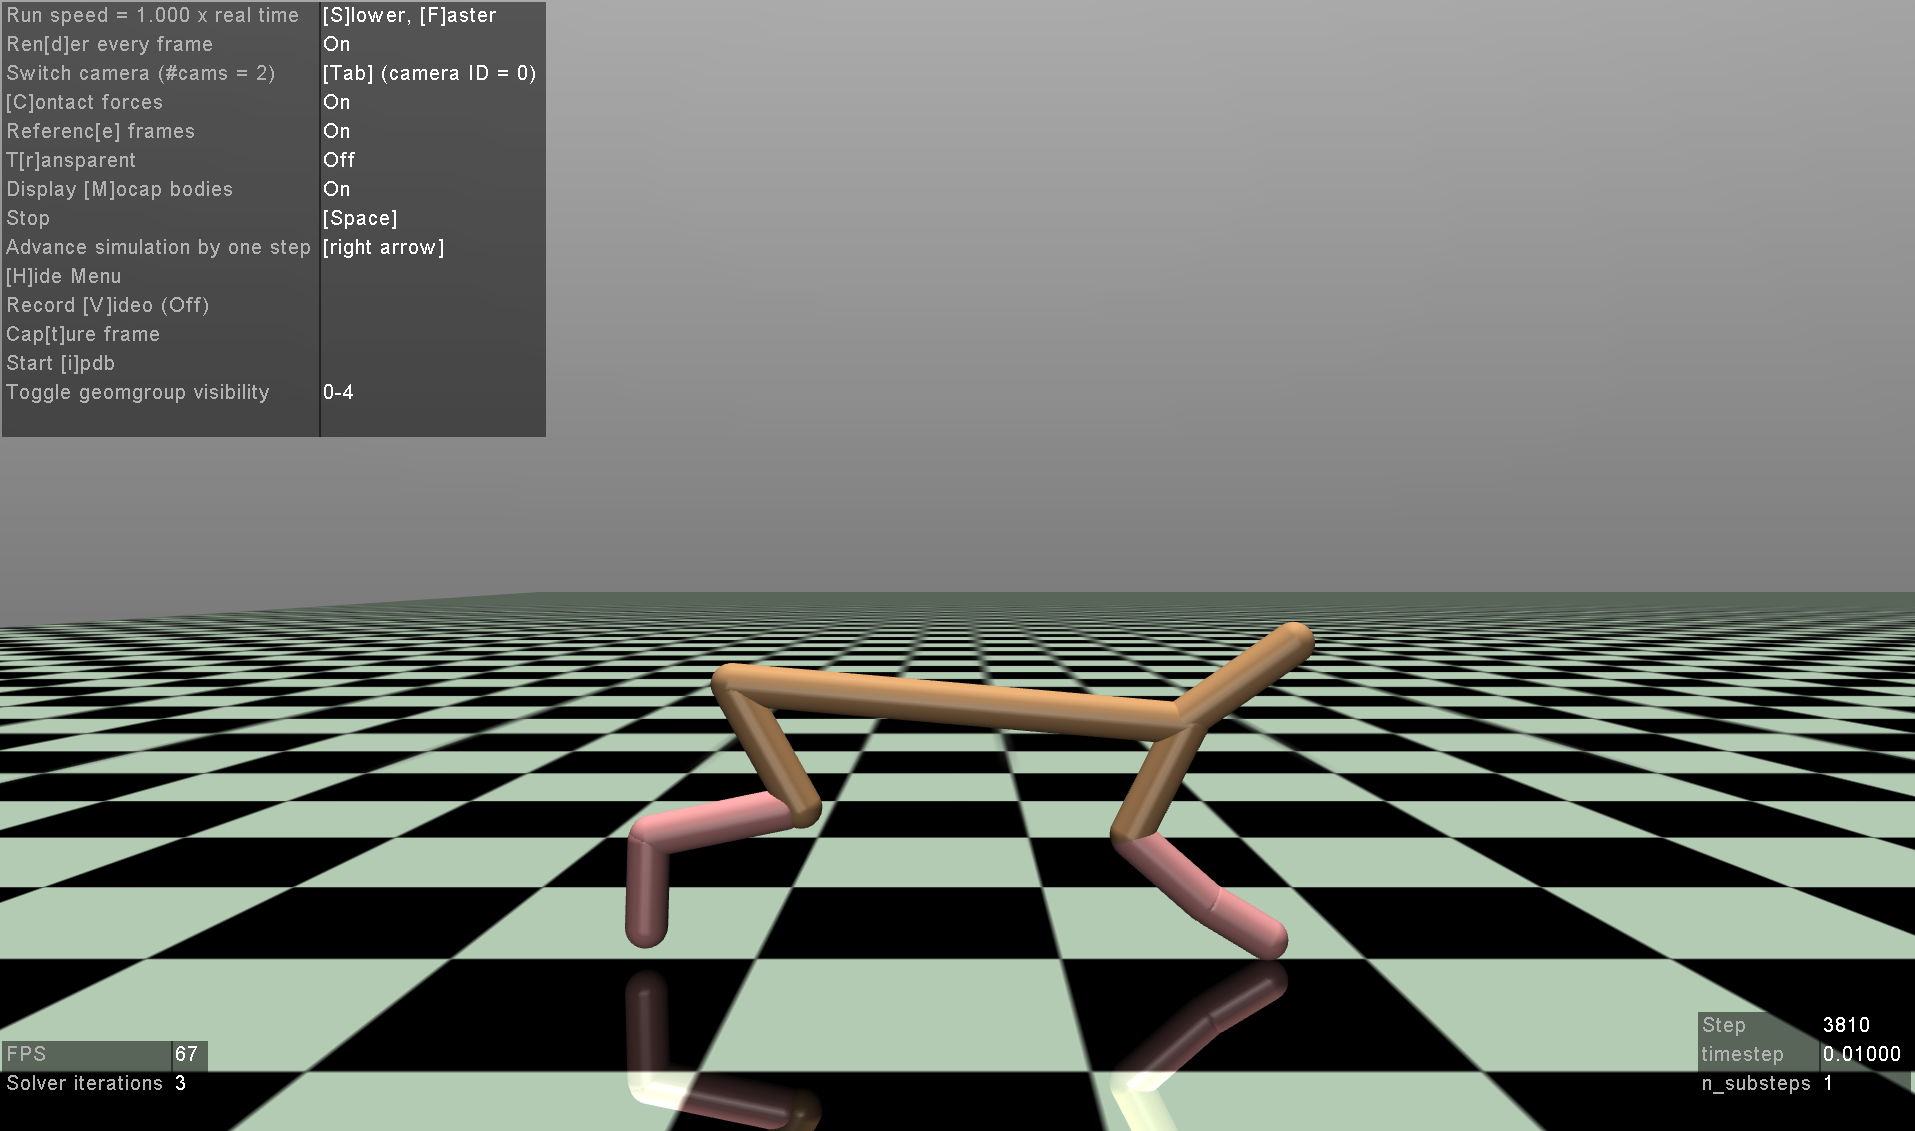
\includegraphics[height=6.5cm]{slika10}
  \caption{Prikaz agenta u okruženju \textit{HalfCheetah}}
  \label{slika10}
\end{figure}

\section{Radno okruženje \textit{LunarLander}}
\textit{LunarLander} je računalna igra iz istog paketa i u njoj je cilj sletjeti na tlo bez oštećenja (Slika \ref{slika11}). Kao i prošlo okruženje, za svaki trenutak agentu se predaju neka zapažanja, a on ih prevodi u akcije. U ovom slučaju agent ima osam realnih brojeva koji opisuju stanje igre u svakom trenutku i može se odlučiti za jednu od četiri radnje. Neki od brojeva koji opisuju stanje su trenutna $x$ pozicija, $y$ pozicija, kut pod kojim je letjelica, dodiruju li lijeva ili desna noga tlo, itd. Od mogućih akcija, agent može upaliti donji, lijevi ili desni motor te ne napraviti ništa. U svakom trenutku ovisno o stanju i svojoj odluci dobiva određeni broj bodova. Za svaki otkucaj za koji agent pali motore gubi $0.3$ boda, dok za svaki doticaj jedne od dvije noge s tlom dobiva $10$ bodova. Na ovaj način agent se nagrađuje za što manje korištenje motora i što mekše slijetanje. Dobiva više bodova ako sleti bliže sredini ekrana gdje mu je označeno mjesto slijetanja. Sredina ekrana uvijek ima ravnu podlogu i nalazi se na koordinatama $(0, 0)$, dok se okolina može mijenjati. Na kraju izvođenja, agent dobije $100$ bodova ako se uspješno zaustavio ili izgubi $100$ ako se sudario. Osim što se okruženje može mijenjati, letjelica može započeti pod drugačijim kutem i početnom brzinom. Igra se smatra riješenom kada jedan agent u sto različitih pokretanja postigne u prosjeku $200$ bodova po pokušaju. U sljedećem poglavlju provedena su ispitivanja za opisane probleme i analizirana je efikasnost algoritma u stvaranju strategije igranja za iste.

\begin{figure}
  \centering
  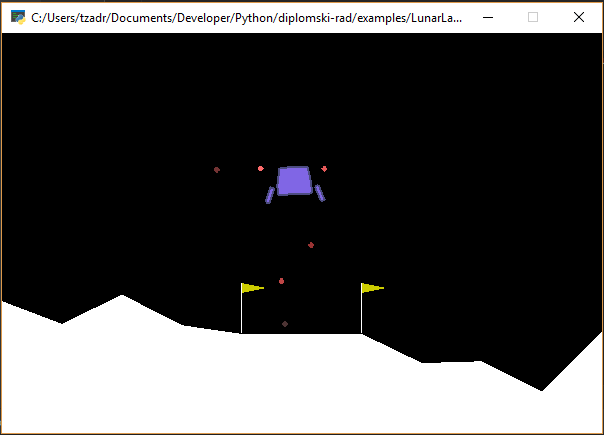
\includegraphics[height=8cm]{slika11}
  \caption{Prikaz agenta u okruženju \textit{LunarLander}}
  \label{slika11}
\end{figure}

\chapter{Ispitivanje}
U ovom poglavlju opisani su rezultati izvođenja za probleme predstavljene u drugom poglavlju.

\section{Problem konstrukcije XOR vrata}
U prethodnom poglavlju opisana je jednakost \ref{jednakost3} kojom se računa dobrota svake jedinke za ovaj problem. U isječku koda \ref{kod19} prikazano je ostvarenje te formule unutar metode \textit{evaluate} kojom se računa dobrota svake jedinke. Metoda prima referencu na jedinku te konstruira fenotip koji je opisan jedinkinim genima. Fenotipu se za sva četiri slučaja problema predaju ulazi, nakon čega se uzima izlaz iz mreže. Pomoću izlaza iz fenotipa računamo pogrešku i time dobrotu jedinke. Ako mreža vrati točan rezultat za sva četiri slučaja spremamo informaciju da je okruženje riješeno. Na glavnom programu je da provjeri tu zastavicu ako želi zaustaviti izvođenje algoritma.

\begin{lstlisting}[frame=single, label=kod19, caption=Izvorni tekst metode \textit{evaluate} za problem konstrukcije XOR vrata]
def evaluate(self, individual):
	# track number of evaluations made
	self.evaluations += 1

	# create phenotype from individual's connection and node genes
	phenotype = Phenotype(individual.connections.values(), individual.nodes.values())

	correct_solutions = True
	fitness = 4

	# for every one of four different cases feed the network input and calculate error based on the output
	for observation, solution in zip(self.observations, self.solutions):
		phenotype.flush()
		output = phenotype.forward(observation)
		result = output[0]

		correct_solutions = correct_solutions and round(result) == solution
		fitness -= (solution - result)**2

	# if solution made no errors the environment is considered solved
	self.solved = self.solved or correct_solutions
	return fitness
\end{lstlisting}

Cilj ovog problema je usporediti rezultate dobivene implementacijom ostvarenom u okviru ovog rada s rezultatima istog problema iz rada u kojem je algoritam originalno predložen \citep{rad5}. Autorima rada trebalo je na sto pokretanja u prosjeku 32 generacije da nađu rješenje, a genom koji rješava problem u prosjeku ima 2.35 skrivena čvora. U ispitivanju predložene implementacije algoritma imitirani su hiperparametri iz originalnog rada. S tim postavkama ova implementacija u sto pokretanja pronalazi rješenje u prosječno 24 generacije, što je za četvrtinu manje vremena. Također, najbolja rješenja ovog ostvarenja imaju u prosjeku 1.08 skrivena čvora, što je čak duplo bolje. Važno je napomenuti da optimalno rješenje ovog problema ima jedan skriveni čvor, što znači da se ova implementacija jako približila optimalnom rješenju. U oba ispitivanja rješenje je pronađeno u svih sto pokretanja, gdje je najduže izvođenje originalnog rada bilo 90 generacija, a ovog skoro trećinu manje, 65 generacija. Više informacija o izvođenjima prikazano je u tablici \ref{tablica2}. Ova tablica sadrži informacije o izvođenju i varijante predloženog algoritma koja ima zaseban ulaz za pristranost.

\subsection{Pristranost u čvorovima}
U prethodnom poglavlju spomenuto je da originalni rad izvodi pristranost tako da prilikom izvođenja ima još jedan ulaz u mrežu kojem je vrijednost uvijek $1$. Na ovaj način veze iz ovog čvora u bilo koji drugi funkcioniraju isto kao pristranost u jednostavnim neuronima. Ova implementacija ne sadrži taj ulaz zato što je pristranost uvedena direktno u čvorove. U tablici \ref{tablica2} vidi se da varijanta ove izvedbe sa zasebnim ulazom za pristranost ostvaruje puno lošije rezultate, i od originalne implementacije i od predložene. Algoritam u sto izvođenja ne nalazi rješenje problema unutar sto generacija u čak šest slučajeva. U ostalih 94, ostvarenje pronalazi rješenje s prosječno 1.19 skrivena čvora, što nije puno lošije od predložene varijante, ali ga pronalazi u prosječno 44 generacije, što je skoro duplo duže. Pretpostavka zašto ova varijanta postiže lošije rezultate je to što, ako algoritam ima poseban ulaz za pristranost, pristranost u čvor će moći biti dodana tek kada se stvori nova veza između tog ulaza i čvora. Pristranost je bitan parametar neurona te se njegova vrijednost treba prilagođavati puno češće nego što se dodaju nove veze. Zbog toga je u predloženoj implementaciji odlučeno pristranost u čvorovima prilagođavati na sličan način i približnom učestalošću kao i težine veza. S ovom promjenom algoritam je u stanju postići puno bolje rezultate, kao što je vidljivo u tablici \ref{tablica2}.

\begin{table}
\resizebox{\textwidth}{!}{%
\begin{tabular}{|cc|rrr|}
\hline
\multicolumn{2}{|c|}{\textbf{Problem konstrukcije XOR vrata}} & \multicolumn{1}{c}{\cellcolor[HTML]{C9DAF8}\textbf{\begin{tabular}[c]{@{}c@{}}Originalna implementacija\\ (poseban ulaz za pristranost)\end{tabular}}} & \multicolumn{1}{c}{\cellcolor[HTML]{C9DAF8}\textbf{\begin{tabular}[c]{@{}c@{}}Imitacija originalne implementacije\\ (poseban ulaz za pristranost)\end{tabular}}} & \multicolumn{1}{c|}{\cellcolor[HTML]{C9DAF8}\textbf{\begin{tabular}[c]{@{}c@{}}Predložena implementacija\\ (pristranost ugrađena u čvorove)\end{tabular}}} \\ \hline
\cellcolor[HTML]{F9CB9C} & \cellcolor[HTML]{FCE5CD}Prosječno & 4,755 (32 generacije) & 6,701 (44 generacije) & 3,734 (24 generacije) \\
\cellcolor[HTML]{F9CB9C} & \cellcolor[HTML]{FCE5CD}Standardna devijacija & 2,553 & 2,997 & 1,417 \\
\multirow{-3}{*}{\cellcolor[HTML]{F9CB9C}Broj evaluacija} & \cellcolor[HTML]{FCE5CD}Najgore pokretanje & 13,459 (90 generacija) & - & 9,891 (65 generacija) \\ \cline{1-2}
\cellcolor[HTML]{F9CB9C} & \cellcolor[HTML]{FCE5CD}Prosječno & 2.35 & 1.19 & 1.08 \\
\multirow{-2}{*}{\cellcolor[HTML]{F9CB9C}Broj skrivenih čvorova} & \cellcolor[HTML]{FCE5CD}Standardna devijacija & 1.11 & 0.42 & 0.31 \\ \cline{1-2}
\cellcolor[HTML]{F9CB9C}Broj aktivnih veza & \cellcolor[HTML]{FCE5CD}Prosječno & 7.48 & 6.64 & 5.12 \\ \cline{1-2}
\multicolumn{2}{|c|}{\cellcolor[HTML]{FCE5CD}\begin{tabular}[c]{@{}c@{}}Broj pokretanja u koliko je algoritam\\ pronašao rješenje u 100 generacija\end{tabular}} & 100/100 & 94/100 & 100/100 \\ \hline
\end{tabular}%
}
\caption{Prikaz podataka o izvršavanju algoritma na problemu konstrukcije XOR vrata}
\label{tablica2}
\end{table}

\section{Optimiranje strategije hodanja u simulaciji \textit{HalfCheetah}}
Za ovaj problem metodu za evaluaciju jedinke trebalo je prilagoditi da odgovara načinu rada biblioteke koja se koristi za pokretanje simulacije. U izvornom kodu isječka \ref{kod20} opisana je ta metoda. Glavna promjena je interakcija s objektom \textit{env} koji predstavlja instancu igre kreirane uz pomoć programske biblioteke \textit{gym} koja je opisana u prethodnom poglavlju. Metoda nakon konstrukcije fenotipa koristi objekt \textit{env} kako bi započela novu igru te prikupljala zapažanja i slala akcije agenta. Kako je prethodno opisano, obzervacije predstavljaju ulaz u neuronsku mrežu, to jest fenotip, a izlaz iz te mreže predstavlja akciju koju agent poduzima. Svaki puta kada agent napravi korak, okruženje osim zapažanja vraća i nagradu i zastavicu koja označava je li igra gotova. Nagrade iz svakog koraka se akumuliraju kako bi se dobila dobrota agenta, a kada je zastavica za kraj igre gotova petlja se može zaustaviti i vratiti do tad akumuliranu količinu nagrada, to jest dobrotu jedinke.

\begin{lstlisting}[frame=single, label=kod20, caption=Izvorni tekst metode \textit{evaluate} za problem optimiranja strategije hodanja u simulaciji \textit{HalfCheetah}]
def evaluate(self, individual, fixed_seed=True, render=False):
	# create phenotype from individual's connection and node genes
	phenotype = Phenotype(individual.connections.values(), individual.nodes.values())

	fitness = 0

	if fixed_seed:
		# ensures every run starts with same observation
		self.env.seed(self.seed)

	# start new game
	observation = self.env.reset()
	while True:
		if render:
			# displays game state on screen
			self.env.render()

		# feed forward neural network with observation
		output = phenotype.forward(observation)
		# scale output to get action
		action = utility.scale(output, self.env.action_space.low, self.env.action_space.high)
		# take step with given action
		observation, reward, done, info = self.env.step(action)

		# accumulate rewards to get individual's fitness
		fitness += reward

		# stop if game is over
		if done:
			break

	return fitness
\end{lstlisting}

Postavke hiperparametara za ovaj problem ne razlikuju se mnogo od prethodnog problema. Promijenjene su jedino tražena veličina populacije te vjerojatnost generiranja novih veza i čvorova, koje u ovom ispitivanju imaju duplo veću vrijednost. Veća populacija potrebna je zato što je domena ovog problema puno veća i potrebno ju je bolje pretraživati. Također, veća populacija ostavlja i više slobode kod dodatnih mutacija. Sve ostale postavke su nepromijenjene. Kako bi ispitivanje bilo olakšano svako pokretanje simulacije počinje iz istog početnog stanja. Na ovaj način osiguran je determinizam, to jest svako pokretanje simulacije s istim fenotipom dat će isti rezultat. U sljedećem podpoglavlju je opisano kako pokretanje s nasumičnim početnim stanjem utječe na rad algoritma.

Rezultati izvođenja algoritma na ovom problemu prikazani su u tablici \ref{tablica3}. Kao što je vidljivo iz pet pokretanja algoritma, najbolji agent je u prosjeku postizao rezultat od $2,146.28$. Na internetu nisu dostupni dobro opisani rezultati drugih rješenja ovog problema, pa nije moguće ovaj rezultat saviti u perspektivu, ali po samoj motorici agenta moguće je zaključiti da agent u većini slučajeva upadne u lokalni optimum iz kojeg ne može izaći. Naime, prilikom trčanja agent ne miče noge efikasno kako bi iskoristio raspon koji može prijeći s njima. Kako je opisano u prethodnom poglavlju, agent upravlja robotom u obliku geparda, stoga ima noge s tri članka: natkoljenica, potkoljenica te stopalo. Agenti u pitanju trče tako da jako brzo kreću stopala, dok im natkoljenica i potkoljenica uglavnom miruju. Koliko god brzo radili, agenti tako neće moći nikada trčati onoliko brzo kolikom bi mogli da koriste i preostala dva dijela noge. Bitno je napomenuti da je poželjno da agent što brže trči jer se dobrota mjeri kao pređena udaljenost u određenom periodu, to jest u određenom broju poteza. U ostatku poglavlja analizirano je korištenje turnirske selekcije umjesto nasumičnog odabira roditelja.

\begin{table}
\resizebox{\textwidth}{!}{%
\begin{tabular}{|cc|rrrrr|rr|}
\cline{1-8}
\textbf{Postavke} & \textbf{\begin{tabular}[c]{@{}c@{}}Najbolja jedinka\\ nakon 100 generacija\end{tabular}} & \multicolumn{1}{c}{\cellcolor[HTML]{C9DAF8}\textbf{\begin{tabular}[c]{@{}c@{}}Pokretanje\\ 1\end{tabular}}} & \multicolumn{1}{c}{\cellcolor[HTML]{C9DAF8}\textbf{\begin{tabular}[c]{@{}c@{}}Pokretanje\\ 2\end{tabular}}} & \multicolumn{1}{c}{\cellcolor[HTML]{C9DAF8}\textbf{\begin{tabular}[c]{@{}c@{}}Pokretanje\\ 3\end{tabular}}} & \multicolumn{1}{c}{\cellcolor[HTML]{C9DAF8}\textbf{\begin{tabular}[c]{@{}c@{}}Pokretanje\\ 4\end{tabular}}} & \multicolumn{1}{c|}{\cellcolor[HTML]{C9DAF8}\textbf{\begin{tabular}[c]{@{}c@{}}Pokretanje\\ 5\end{tabular}}} & \multicolumn{1}{c}{\cellcolor[HTML]{A4C2F4}\textbf{Prosječno}} & \multicolumn{1}{c|}{\cellcolor[HTML]{A4C2F4}\textbf{\begin{tabular}[c]{@{}c@{}}Standardna\\ devijacija\end{tabular}}} \\ \hline
\cellcolor[HTML]{F9CB9C} & \cellcolor[HTML]{FCE5CD}Rezultat & 1,438 & 2,193 & 2,500 & 2,632 & 1,999 & 2,146 & 420 \\
\cellcolor[HTML]{F9CB9C} & \cellcolor[HTML]{FCE5CD}Broj čvorova & 5 & 2 & 4 & 1 & 10 & 4.40 & 3.14 \\
\multirow{-3}{*}{\cellcolor[HTML]{F9CB9C}\begin{tabular}[c]{@{}c@{}}Visoka stopa smrtnosti (80\%)\\ \&\\ Nasumičan odabir roditelja\end{tabular}} & \cellcolor[HTML]{FCE5CD}Broj veza & 110 & 104 & 107 & 100 & 112 & 106.60 & 4.27 \\ \hline
\cellcolor[HTML]{F9CB9C} & \cellcolor[HTML]{FCE5CD}Rezultat & 1,505 & 2,939 & 1,333 & 1,866 & 2,452 & 2,019 & 599 \\
\cellcolor[HTML]{F9CB9C} & \cellcolor[HTML]{FCE5CD}Broj čvorova & 8 & 3 & 6 & 7 & 8 & 6.40 & 1.85 \\
\multirow{-3}{*}{\cellcolor[HTML]{F9CB9C}\begin{tabular}[c]{@{}c@{}}Niska stopa smrtnosti (0\%)\\ \&\\ Turnirska selekcija (k = 5)\end{tabular}} & \cellcolor[HTML]{FCE5CD}Broj veza & 72 & 91 & 84 & 72 & 67 & 77.20 & 8.89 \\ \hline
\end{tabular}%
}
\caption{Prikaz podataka o izvršavanju algoritma na problemu optimiranje strategije hodanja u simulaciji \textit{HalfCheetah}}
\label{tablica3}
\end{table}

\subsection{\textit{Turnirska selekcija}}
U tablici \ref{tablica3} također je moguće vidjeti rezultate pokretanja i za drugi slučaj koji je predmet ovog potpoglavlja. U prethodnom poglavlju opisana je turnirska selekcija te kako se ona razlikuje od nasumičnog odabira. Ovo ostvarenje, kao i originalni algoritam \citep{rad5}, općenito ima visoku stopu smrtnosti u populaciji, toliku da se čak 80\% populacije nema pravo razmnožavati. Na ovaj način pokušava se osigurati da se razmnožavaju samo što bolje jedinke. Ovo je dosta agresivan način kako bi se postigao ovaj učinak, stoga je ovdje predloženo korištenje turnirske selekcije. Kao što je rečeno, turnirska selekcija odabire malu količinu jedinki koje će se međusobno nadmetati. Tako se postiže isti rezultat, nagrađuje se bolje jedinke, ali odabir jedinki za turnirsku selekciju je nasumičan, stoga je moguće da pobjede i neke jedinke koje inače ne bi imale pravo na križanje. Kako bi pritisak na populaciju i dalje ostao velik, veličina turnira povećana je na $5$, što znači da su manje šanse da će lošija jedinka pobijediti u turniru. Na tablici \ref{tablica3} je vidljivo da obje varijante postižu približno jednak prosječan rezultat, turnirska selekcija s prosječnim rezultatom od $2,019.09$ u odnosu na nasumičnu s rezultatom $2,146.28$. Turnirska selekcija stvara jedinke s malo većim brojem čvorova, prosječno $6.4$ u odnosu na nasumičnu s $4.4$, ali rješenja imaju manji broj veza, prosječno $77.2$ u odnosu na $106.6$. Budući da obje varijante zapinju u istom lokalnom optimumu teško je odrediti koja varijanta je bolja.

\section{Optimiranje strategije igranja igre \textit{LunarLander}}
Ovaj problem najsličniji je situaciji u kojoj će se algoritam pronaći prilikom stvaranja strategije igranja u većini računalnih igara. Postavke odabrane za ovo ispitivanje iste su kao postavke korištene za ispitivanje optimiranja strategije hodanja u simulaciji \textit{HalfCheetah}. Metoda koja evaluira ovaj problem gotovo je ista kao i za prethodni problem, jedina razlika je ta što objekt \textit{env} mora biti inicijaliziran s drugim ključem igre, to jest s ključem igre \textit{LunarLander}. Jedno pokretanje ovog algoritma u brzini kojoj bi čovjek igrao traje u prosjeku jedan cijeli dan prije nego algoritam pronađe rješenje. Bitno je uzeti u obzir da je ovo bez paralelizacije evaluiranja jedinki. U tablici \ref{tablica4} mogu se vidjeti rezultati pet pokretanja algoritma. Algoritam pronalazi rješenje, ali mu je standardna devijacija broja generacija prije pronalaska rješenja dosta velika. U ostatku poglavlja prikazani su grafovi s detaljnijim podacima o izvođenju. Svi grafovi u ostatku poglavlja odgovaraju istom pokretanju algoritma.

\begin{table}
\resizebox{\textwidth}{!}{%
\begin{tabular}{|cc|rrrrr|rr|}
\hline
\multicolumn{1}{|l}{} & \textbf{} & \multicolumn{1}{c}{\cellcolor[HTML]{C9DAF8}\textbf{\begin{tabular}[c]{@{}c@{}}Pokretanje\\ 1\end{tabular}}} & \multicolumn{1}{c}{\cellcolor[HTML]{C9DAF8}\textbf{\begin{tabular}[c]{@{}c@{}}Pokretanje\\ 2\end{tabular}}} & \multicolumn{1}{c}{\cellcolor[HTML]{C9DAF8}\textbf{\begin{tabular}[c]{@{}c@{}}Pokretanje\\ 3\end{tabular}}} & \multicolumn{1}{c}{\cellcolor[HTML]{C9DAF8}\textbf{\begin{tabular}[c]{@{}c@{}}Pokretanje\\ 4\end{tabular}}} & \multicolumn{1}{c|}{\cellcolor[HTML]{C9DAF8}\textbf{\begin{tabular}[c]{@{}c@{}}Pokretanje\\ 5\end{tabular}}} & \multicolumn{1}{c}{\cellcolor[HTML]{A4C2F4}\textbf{Prosječno}} & \multicolumn{1}{c|}{\cellcolor[HTML]{A4C2F4}\textbf{\begin{tabular}[c]{@{}c@{}}Standardna\\ devijacija\end{tabular}}} \\ \hline
\cellcolor[HTML]{F9CB9C} & \cellcolor[HTML]{FCE5CD}Broj čvorova & 8 & 6 & 9 & 5 & 5 & 6.60 & 1.62 \\
\multirow{-2}{*}{\cellcolor[HTML]{F9CB9C}Najbolja jedinka} & \cellcolor[HTML]{FCE5CD}Broj aktivnih veza & 47 & 48 & 57 & 48 & 42 & 48.40 & 4.84 \\ \cline{1-2}
\multicolumn{2}{|c|}{\cellcolor[HTML]{FCE5CD}Broj generacija prije pronalaska rješenja} & 88 & 68 & 103 & 80 & 42 & 76.20 & 20.54 \\ \hline
\end{tabular}%
}
\caption{Prikaz podataka o izvršavanju algoritma na problemu optimiranje strategije igranja u videoigri \textit{LunarLander}}
\label{tablica4}
\end{table}

\subsection{Problem nasumičnog pokretanja}
Jedan bitan aspekt ovog okruženja je što agent mora u sto generacija postići dobar rezultat kako bi se problem smatrao riješenim. Budući da je to skup proces, teži se izbjeći potrebu da se u svakoj generaciji svaku jedinku ispituje sto puta. Pogotovo zato što je prilično sigurno da jedinke koje postignu loš rezultat kroz sto pokretanja neće moći to lako ispraviti. Zbog toga se u svakoj generaciji predloži samo najbolju jedinku za rješenje problema. Tom logikom, ako je u populaciji $N$ jedinki, ukupan broj evaluacija u toj generaciji bi umjesto $N * 100$ trebao bi biti $N + 100$. Sto različitih pokretanja koja su potrebna za utvrditi je li jedinka zadovoljavajuća izvršavaju se na kraju generacije i osim što su uvjet za zaustavljanje algoritma nisu uzete kod daljnje evaluacije jedinke.

Mana ovakvog pristupa je što se najbolja jedinka u generaciji treba jako pažljivo izabrati, kako bi izbjegli situaciju u kojoj jedinka koja je možda bolja u ovom pokretanju nije bolja od drugoplasirane u ostalih 99. Stoga je važna odluka bila koja početna stanja koristiti prilikom evaluacije jedinke. U ovom slučaju postoje tri mogućnosti. Prva, najjednostavnija, bi bila da je početno stanje kod svakog pokretanja nasumično. To bi značilo da bi svake dvije jedinke u istoj generaciji prilikom evaluacije počinjale iz različitih početnih pozicija. Druga opcija je da je početno stanje u svim generacijama i za sve jedinke isto. Dakle, jedinka bi se u svakoj generaciji ispitivala na istom pokušaju, ali bi se jedinka koja je najbolja u svakoj generaciji i dalje morala pokrenuti za sto nasumičnih početnih stanja. Treća, zadnja opcija, je da je početno stanje za cijelu generaciju isto, ali da se mijenja iz generacije u generaciju. Tako sve jedinke u generaciji bile bi ispitane na istom okruženju, ali bi se to okruženje mijenjalo u svakoj generaciji kako bi se jedinke ispitivale na raznolikim slučajevima.

Prva opcija nije uspjela naći rješenje u sto generacija. Zbog toga što se svaka jedinka ispituje na nasumičnom početnom stanju na kraju generacije gotovo je nemoguće utvrditi koja jedinka je objektivno najbolja. U ovom načinu vrlo je vjerojatno da je jedinka koja je dobila najveći rezultat zapravo nasumično bila pokrenuta na vrlo lakom početnom stanju i bez puno znanja mogla je postići veći rezultat od neke koja je u prosjeku bolja od nje, ali je pokrenuta na vrlo teškom početnom stanju. Zbog ovoga populacija je vrlo slabo napredovala i čak u situacijama kada je postojalo potencijalno zadovoljavajuće rješenje u populaciji moguće je da je zaobiđeno zbog jedinke koja je nasumično postigla dobar rezultat.

Prilikom pokretanja druge opcije nije dobiven puno bolji rezultat. Algoritam također nije mogao naći rješenje unutar sto generacija. U ovom slučaju funkcija najbolje dobrote je za razliku od prve opcije monotono rasla, zato što je populacija kroz generacije zapravo učila postati ekspert za to određeno početno stanje. Štoviše, populacija je naučila odlično riješiti to specifično okruženje, ali zbog manjka varijacije u ispitivanju jedinke jednostavno nisu bile dovoljno robusne, tj. nisu se naučile prilagođavati različitim početnim situacijama.

Zadnja opcija je kombinacija prve dvije. Ispitivanje svake generacije na istom početnom stanju omogućilo je puno veću sigurnost odabira najbolje jedinke u generaciji. Ovaj problem nije u potpunosti riješen, ali ako se ispituje sve jedinke na istom slučaju veća je vjerojatnost da će ona s najboljim rezultatom biti bolja i u ostalih 99. Osim toga, odabir novog početnog stanja za svaku generaciju uvelo je varijaciju u algoritam. Ispitivanje jedinki na različitim početnim stanjima stvara puno robusnije jedinke. Algoritam koji je pokrenut s ovom postavkom u jednom pokretanju pronašao je rješenje u malo 78 generacija. Funkcija najbolje dobrote prikazana je crvenom bojom na slici \ref{slika13}. Ona zbog ove opcije više nije monotona, ali u prosjeku se može vidjeti da funkcija ipak raste. Zanimljivo je primijetiti da u početku funkcija puno više varira, zbog toga što su neka početna stanja teža, a neka lakša. Kasnije, kada jedinke postaju robusnije, funkcija ima puno manju standardnu devijaciju. U sljedećem potpoglavlju prikazano je još nekoliko grafova s informacijama dobivenim iz istog pokretanja.

\begin{figure}
  \centering
  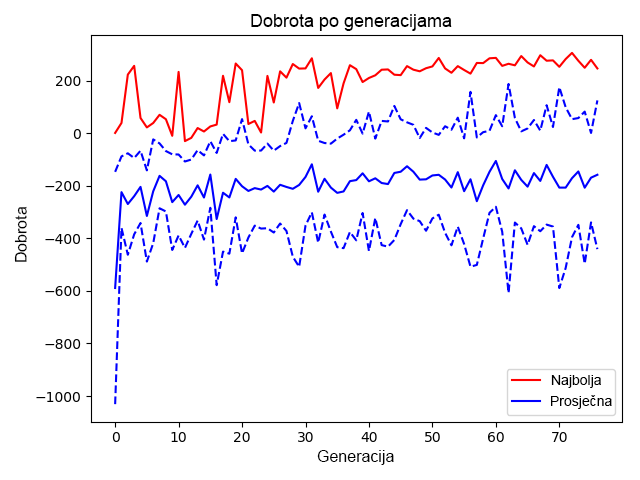
\includegraphics[height=7cm]{slika13}
  \caption{Funkcija najbolje i prosječne dobrote po generacijama}
  \label{slika13}
\end{figure}

\begin{figure}
  \centering
  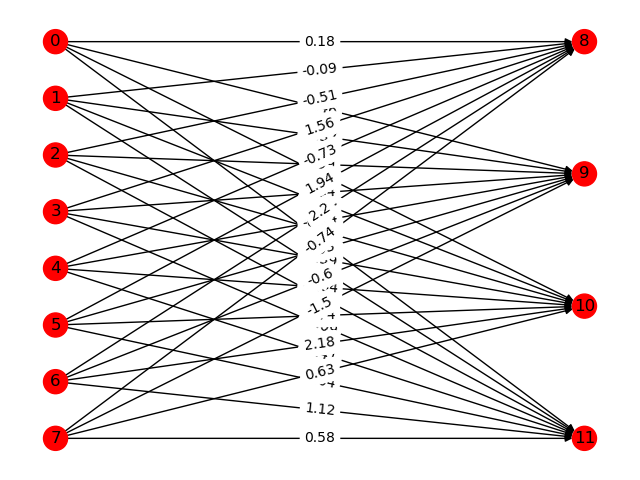
\includegraphics[height=6cm]{slika14}
  \caption{Prikaz neuronske mreže najbolje jedinke u prvoj generaciji}
  \label{slika14}
\end{figure}

\begin{figure}
  \centering
  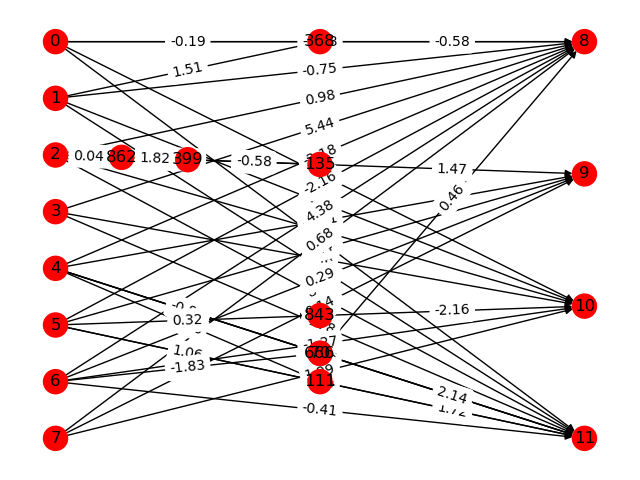
\includegraphics[height=6cm]{slika15}
  \caption{Prikaz neuronske mreže najbolje jedinke koja je riješila problem}
  \label{slika15}
\end{figure}

\subsection{Ostali rezultati}
Na slikama su prikazane struktura najbolje jedinke u prvoj generaciji (Slika \ref{slika14}) i struktura jedinke koja je na kraju riješila problem (Slika \ref{slika15}). Po ovim slikama vidi se kako se kroz generacije struktura povećava. Na jednoj vezi najbolje jedinke (Slika \ref{slika15}) vide se tri čvora u koje se ne uključuje nijedna druga veza. Bilo bi idealno naći način da se ovakve redundancije izbjegnu. Rast broja čvorova i veza može se vidjeti na slici \ref{slika16}. Može se primijetiti da iako su im vjerojatnosti za stvaranje različite, ove dvije brojke su korelirane zato što bez dovoljno čvorova nije moguće stvarati ni dodatne veze.

\begin{figure}
  \centering
  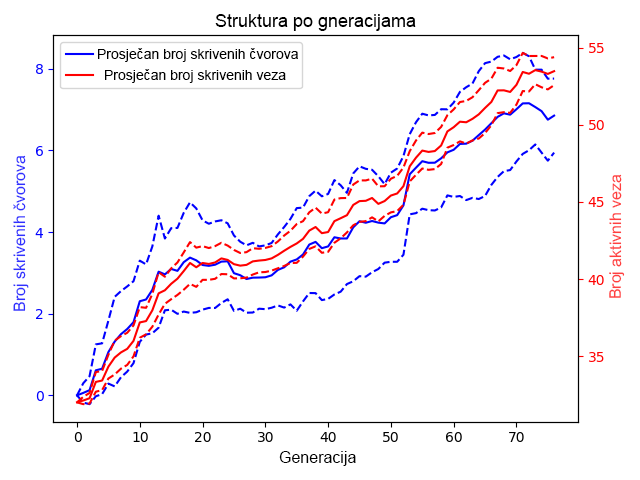
\includegraphics[height=7cm]{slika16}
  \caption{Prikaz rasta broja čvorova i veza kroz generacije}
  \label{slika16}
\end{figure}

Kako bi postepeni napredak strukture jedinki bio bolje vidljiv, najbolje je pogledati udio vrsta kroz generacije prikazan na slici \ref{slika17}. Može se vidjeti kako veće vrste rastu te kroz dvadesetak generacija postepeno umiru, a kako one umiru postepeno se stvaraju nove vrste čime se ciklus nastavlja. Ako se usporedi s grafom na slici \ref{slika16} vidljivo je kako na početku, kada je struktura još jednostavna, postoji samo jedna vrsta. Nakon inicijalnih mutacija broj vrsta jako poraste, zbog čega se smanji prosječni broj jedinki po vrsti, a složenost strukture poraste. Razlog iz kojeg se ovo događa je kompenzacija praga kompatibilnosti kojeg se može vidjeti na slici \ref{slika18}. Prag kompatibilnosti definira koliko daleko jedinka može biti od predstavnika vrste da bi se smatrala dijelom te vrste. Zbog toga, ako je prag kompatibilnosti velik, vrste će obuhvaćati raznolikije jedinke. Stoga, ako je prag kompatibilnosti velik i vrste će biti veće te će broj vrsta biti manji. Problem eksplozije broja vrsta nastaje zato što na početku, kada algoritam još nema vremena stvoriti dovoljno raznolike jedinke, prag kompatibilnosti pokušava to kompenzirati tako da se smanjuje. Jednom kada počinju nastajati promjene prag kompatibilnosti je već mali te nastaje puno vrsta. Nakon što se prođe željeni prag broja vrsti prag se ponovo povećava te se i broj vrsti stabilizira. Na slici \ref{slika19} se vidi kako prosječna udaljenost jedinki u početku brzo raste, ali se onda donekle stabilizira. Iako je potrebno bolje definirati način na koji se prag kompatibilnosti podešava, reguliranje broja vrsti na ovaj način pokazalo je bolje rezultate u problemu konstrukcije XOR vrata.

\begin{figure}
  \centering
  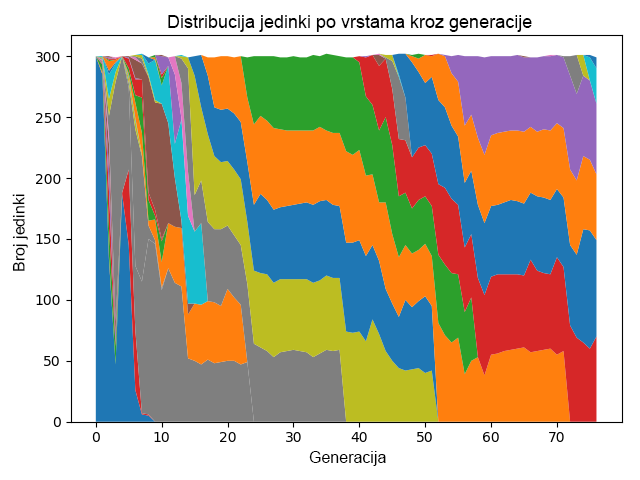
\includegraphics[height=7cm]{slika17}
  \caption{Vizualni prikaz udjela vrsta u populaciji kroz generacije}
  \label{slika17}
\end{figure}

\begin{figure}
  \centering
  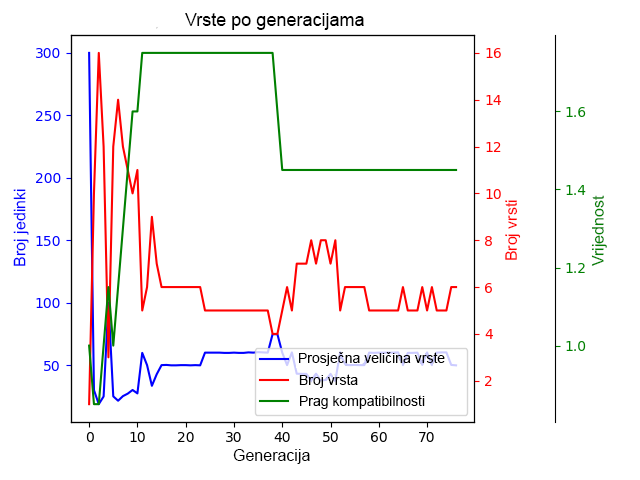
\includegraphics[height=7cm]{slika18}
  \caption{Korelacija broja vrsti i prosječne veličine vrste s pragom kompatibilnosti}
  \label{slika18}
\end{figure}

\begin{figure}
  \centering
  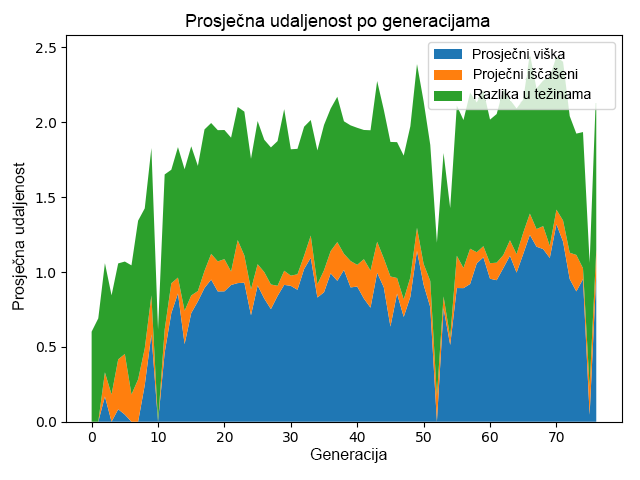
\includegraphics[height=7cm]{slika19}
  \caption{Korelacija broja vrsti i prosječne veličine vrste s pragom kompatibilnosti}
  \label{slika19}
\end{figure}

\subsection{Izlazak iz lokalnog optimuma}
Veliki izazov odabira postavki je znati koje omogućavaju konvergenciju globalnom, a ne samo lokalnom optimumu. U nekoliko pokretanja ovog problema agenti su zapinjali u istom lokalnom optimumu. U pravilima okruženja, agent u svakom trenutku u kojem nogom dodiruje tlo dobiva $10$ bodova. Događalo se da su agenti naučili mirno sletjeti na tlo, ali umjesto da isključe sve motore i prime veliku nagradu kontinuirano su palili lijeve i desne motore kako bi se nastavili gibati dodirujući tlo i time primati malu količinu bodova. Ovime su zapeli u lokalnom optimumu jer su u tom trenutku to bili najbolji rezultati, ali im je trebalo dosta generacija da bi naučili da je nagrada veća ako se što prije zaustave na tlu.

\chapter{Zaključak}
U ovom radu prikazana je povezanost između videoigara i razvoja umjetne inteligencije. Opisane su karakteristike neuroevolucijskog algoritma promjenjivih topologija, algoritma  neuroevolucije koji, koristeći genetske algoritme, optimizira težine i razvija strukturu umjetnih neuronskih mreža. Na ovaj način mogu se konstruirati strategije igranja igara te je algoritam ispitan na tri različita problema. Problemi su ispitani implementacijom algoritma koja je ostvarena u okviru ovog rada. Ostvarenje je rađeno po uzoru originalne implementacije iz rada u kojem je algoritam predložen \citep{rad5} uz promjene koje su predložene u okviru ovog rada. Iako je kroz dinamičku optimizaciju praga kompatibilnosti i uvođenje pristranosti u genom pokazan napredak u odnosu na originalnu implementaciju \citep{rad5}, algoritam još nije konkurentan modernim metodama potpornog učenja. Neke ideje koje bi se isplatilo razmotriti kako bi se poboljšao rad algoritma su paralelizacija, čuvanje liste inovacija kroz više generacija te manju mutaciju veza i pristranosti što su veze i čvorovi stariji.

Budući da je velika prednost ovog algoritma lakoća implementacije paralelizacije uvelike bi se ubrzalo vrijeme izvođenja kada bi se evaluacije izvodile paralelno. Ovo je jednostavno dodati u predloženu implementaciju i sve što je potrebno je napraviti metodu koja bi se brinula za distribuiranje evaluacija po različitim dretvama i za prikupljanje rezultata evaluacija. Najveći problem je naći ili napraviti okruženje koje bi podržavalo lako paralelno izvođenje. Okruženja koja moraju stvarati prikaz na ekranu često nisu zamišljena da ih se nanovo stvara prilikom svake evaluacije.

Čuvanje lista inovacija tijekom cijelog izvođenja omogućilo bi ne samo da se prepoznaju iste mutacije unutar jedne generacije, nego da se iste strukturalne promjene prepoznaju u svakom trenutku. Ovo bi moglo pomoći jedinkama da se bolje usklade prilikom križanja te da udaljenost između jedinki bude konzistentnija.

Na kraju, manja mutacija starih veza i čvorova pomogla bi kod većih strukturalnih promjena da se algoritam fokusira samo na novonastale veze i čvorove. Naprimjer, veza koja je nastala u prvoj generaciji prošla je puno više iteracija od veze koja je nastala u pedesetoj generaciji. Zbog toga se može reći da su u tom trenutku veće vjerojatnosti da je prva veza bolje prilagođena od nove. U tom slučaju nema potrebe da se obje veze jednako mutiraju, već je moguće napraviti sustav u kojem je korak perturbacije manji što je veza starija.

Zaključno s time, neuroevolucija promjenjivih topologija ovime je pokazala da može konstruirati dovoljno djelotvorna rješenja.

\bibliography{literatura}
\bibliographystyle{fer}

\begin{sazetak}
U radu je opisan razvoj umjetne inteligencije na primjerima računalnih igara. Proučeno je korištenje genetskih algoritama za razvijanje težina i topologije umjetnih neuronskih mreža. Naučene mreže koriste se za stvaranje strategije igranja jednostavnih videoigara. Ostvaren je algoritam u okviru rada koji je onda ispitan na jednostavnim problemima. Analizirana je djelotvornost sustava i razmotreni su sljedeći mogući koraci za unaprjeđenje algoritma.

\kljucnerijeci{neuroevolucija promjenjivih topologija, genetski algoritmi, neuroevolucija, umjetne neuronske mreže}
\end{sazetak}

\engtitle{Application of neuroevolution of augmenting topologies in playing computer games}
\begin{abstract}
In this paper we describe the influence of computer games on the field of artificial intelligence. We cover application of genetic algorithms on optimizing weights and developing structure of artificial neural networks. Trained networks are used to define playing strategies for simple videogames. We implemented the algorithm within the scope of this paper which is then tested on simple problems. We then analyzed it's efficiency and proposed some further improvements.

\keywords{neuroevolution of augmenting topologies, genetic algorithms, neuroevolution, artificial neural networks}
\end{abstract}

\end{document}